\documentclass[letterpaper,10pt]{article}
%\documentclass[a3paper,twocolumn,10pt]{article}
\usepackage[bookmarks]{hyperref}
\usepackage[utf8]{inputenc}
\usepackage[english]{babel}

% sans serif
\renewcommand*{\familydefault}{\sfdefault}

% pictures!
\usepackage{graphicx}
    % \begin{figure}[H][p]
    %     \centering
    %     \includegraphics[width=0.8\textwidth]{image.png}
    %     \caption{Awesome Image}
    %     \label{fig:awesome_image}
    % \end{figure}

% math++
\usepackage{mathtools}
\usepackage{amsfonts}

% compact lists (compactitem, compactenum, compactdesc)
\usepackage{paralist}

% nicer tables
\usepackage{booktabs}

% layout
\usepackage{float}

% chemical equations
\usepackage{mhchem}

% text columns
\usepackage{multicol}

% dummy text
\usepackage{lipsum}

% frames around text
\usepackage{mdframed}

% section style
\usepackage{sectsty}

% margins
\usepackage[top=0.25in, bottom=0.25in, left=0.25in, right=0.25in]{geometry}

% per-section toc
\usepackage[tight,insection]{minitoc}

\mdfsetup{nobreak=false} %, rightline=false, leftline=false}

% style
\restylefloat{table}
\sectionfont{\rmfamily}
\subsectionfont{\rmfamily\centering}

%ceiling/floor. use \ceil*{stuff} to scale symbols
\DeclarePairedDelimiter\ceil{\lceil}{\rceil}
\DeclarePairedDelimiter\floor{\lfloor}{\rfloor}

\renewcommand\thesection{\Roman{section}}

\begin{document}

\begin{center}
\textbf{\huge
  Summary of Colin Ware's ``Information Visualization: Perception for Design''
}
\\
{\Large Hugo Rivera, Spring 2015}
\end{center}

Notes taken for Visualization CSE 476 taught at the New Mexico Institute of Mining and Technology, Spring 2015.

Summarize chapters 1 to 11 and Appendix D.

\dosecttoc
\setlength{\mtcindent}{0pt}
\setcounter{tocdepth}{1}

\begin{multicols}{2}
\tableofcontents
\end{multicols}

\def\stctitle{}

 \section{Chapter 1: Foundations for an applied science of data visualization}

\graphicspath{ {pngs/ch1/} }
%    \begin{figure}[H]
%        \centering
%        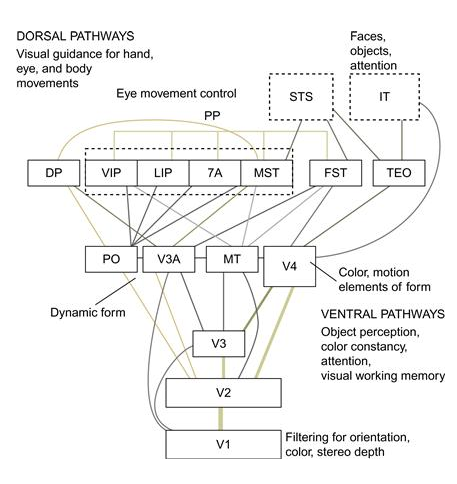
\includegraphics[width=0.4\textwidth]{brain.png}
%        \caption{Macaque monkey brain}
%    \end{figure}


\secttoc


Visualization is the application of vision research to problems of data
analysis. As visualization becomes more important, so does its scientific
understanding. Sensory and arbitrary symbols are split by fundamental
differences, but classification can be difficult. Consistent notation is most
important. This book assumes all humans have more or less the same visual
system.

\begin{mdframed}\begin{multicols}{2}
\subsection{Visualization}
        \begin{figure}[H]
            \centering
            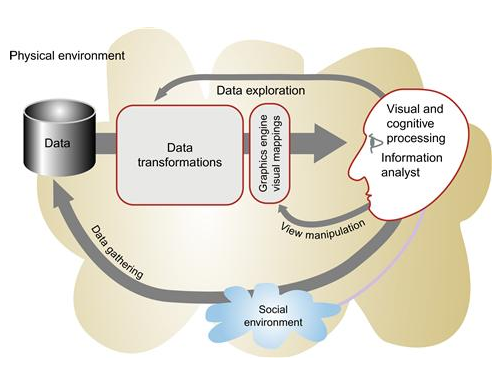
\includegraphics[width=0.3\textwidth]{stages.png}
            \caption{Stages of visualization}
        \end{figure}
\begin{compactdesc}
    \item[Visualization] A graphical representation of data or concepts. Old:
        constructing a visual image in the mind.
    \item[Benefits of visualization]:
        \begin{compactenum}
        \item Comprehend huge amounts of data
        \item Perception of unanticipated, emergent properties
        \item Problems with data become apparent
        \item Understanding of both large-scale and small-scale features
        \item Hypothesis formation is encouraged
        \end{compactenum}
    \item[Visualization stages] form feedback loops in the search for new
        information:
    \item[Data gathering] is the longest feedback loop.
    \item[Visualization] can be highly interactive

        \begin{figure}[H]
            \centering
            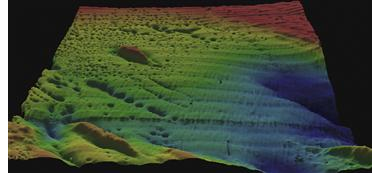
\includegraphics[width=0.25\textwidth]{pasamoquoddy_vis.png}
            \caption{Pasamoquoddy bay scans. A lot of data. Roll of the ship
            was not corrected for.}
        \end{figure}


\end{compactdesc}
\end{multicols}\end{mdframed}

\begin{mdframed}\begin{multicols}{2}
\subsection{Semiotics}

\begin{compactdesc}
\item[Semiotics] the study of making meaning. Signs, analogy, indication,
    designation, metaphor, symbol, communication.
\item[Counter-argument:] diagrams are arbitary, all symbols are learned thus
    one visualization is as good as another regardless of ease of perception.
\item[This debate] helps us decide where visualization science is useful and
    where we should consult a trained designer.
\item[Semiotics of graphics] dominated by non-rigorous philosophers. What is a
    visual language?
\item[Biggest threat] philosophers argue that truth is only so in the context
    of its creators' culture. Meaning is curated by culture. All representations
    have meaning to those trained/raised to know them.
\item[These arguments are rejected] we can have a new semiotics based on
    scientific evidence, not philosopher's claims.
\item[People can interpret] pictures without training clearly (2 studies). The
    outline of an object and the object itself excite similar neural processes.
\end{compactdesc}
\end{multicols}\end{mdframed}




\begin{mdframed}\begin{multicols}{2}
\subsection{Sensory vs Arbitrary}

\begin{compactdesc}
\item[Sensory] is defined here as the aspects of representation that are
    expressive due to the natural perceptual processing power of the brain.
    Full scientific methodology can be applied. Nearly universal.
\item[Arbitrary] is defined here as the aspects of representation that must
    be learned. Interpretive methodology needed.
\item[Example] circles in nearly all cultures represent a bounded region
\item[We reject the idea] that the visual system can adapt to any universe,
    and that our vision is intertwined with this planet.
\item[Many specialized] regions in our brain develop only for their single
    purpose, not a tabula rasa.
\item[Small adaptations] cats raised in a world of only vertical stripes
    develop an unusual number of vertical-edge detectors
\item[Macaque Monkey's] visual system: V1 (orientation, color, stereo depth)
    $\to$ V2 $\to$ V3 $\to$ V4 (Color, motion, elements of form) and other
    systems. Also: object perception, color constancy, attention, visual
    working memory.
\item[Sensory representations] work because they are well matched to the
    first stages of perception.
    \begin{compactenum}
    \item Understanding without training
    \item Resistance to alternate denotation
    \item Sensory immediacy
    \item Cross cultural validity
    \end{compactenum}
\item[Vision researchers and biologists] can test claims about sensory
    representation.
\item[Arbitrary codes] are socially constructured
    \begin{compactenum}
    \item Hard to learn
    \item Easy to forget
    \item Embedded in culture and applications
    \item Formally powerful, can be matched to rigorous languages
    \end{compactenum}
\item[Sensory and arbitary are intertwined] but the visualization designer must
    still be able to apply the science of visualization
\end{compactdesc}

        \begin{figure}[H]
            \centering
            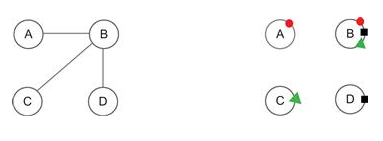
\includegraphics[width=0.3\textwidth]{graph_vis.png}
            \caption{Left visualization is easier to interpret}
        \end{figure}



\end{multicols}\end{mdframed}




\begin{mdframed}\begin{multicols}{2}
    \subsection{Gibson's Affordance theory}

\begin{compactdesc}
\item[Affordances] are possibilities for action that can be percevied
\item[Directly] seen, not inferred from sensory cues.
\item[Action-based] perception!
\item[We do not perceive] points of light and go up from there, our visual
    system works from top to bottom.
\item[Three problems]:
    \begin{compactenum}
    \item Computer graphics are very indirect, detached from the way we
        interact with them
    \item No clear physical affordances in any graphical user interface.
        Buttons are arbitrary
    \item Gibson rejected visual mechanisms. Mistake. Color perception is an inborn
        trait, it is actually a thoroughly studied system, and it is entirely
        bottom-up.
    \end{compactenum}
\end{compactdesc}
    \subsection{A model of perceptual processing}
\begin{compactdesc}
\item[Stage 1: Parallel processing, low-level properties] primitive, specialized
    and fast. Bottom-up, visual salience. If information must be understood
    quickly, here is where optimizations are needed.
\item[Stage 2: Pattern Perception] Rapid processes divide the field into
    regions and simple patterns like contours and regions of shared
    color/texture. Motion. Flexible. Deals with the massive amount of data
    from stage 1 and tunes queries using the higher-level process of attention.
    Slower, serial. One to three objects can be held for a second or two.
\item[Stage 3: Visual working meory] highest level. Sequence of visual
    queries. Only a few objects held at a time. Constructed from the lower
    levels.
\item[Attention] The top-down signal that consolidates and enhances the jobs
    of the visual system. Multifaceted, pervasive.
\end{compactdesc}
\end{multicols}\end{mdframed}




\begin{mdframed}\begin{multicols}{2}
\subsection{Costs and Benefits of Visualization}

\begin{compactdesc}
\item[Must measure value] in some way to optimize a system. Workers will work
    easier, less stress. A scientific discovery could be made.
\item[Cost for user:] time to learn
\item[Benefit for user:] improved cognitive workload
\item[Cost for dev:] time to develop visualization, cost to market,
    manufacture, service
\item[Benefits for dev:] units sold, revenue
\end{compactdesc}

\subsection{Types of data}
\begin{compactenum}
\item entities, relationships, attributes
\item dimensionality: 1,2,3 and up
\item types of numbers
\item uncertainty
\item operations such as arithmetic, merging, removing
\item metadata: data about data, who/what, transforms and uncertainty
\end{compactenum}


\end{multicols}\end{mdframed}


 \section{Chapter 2: Environment, Optics, Resolution, Display}

\graphicspath{ {pngs/ch2/} }



\secttoc

The computer screen is utterly simple when compared to the richness of the
visual world. Remarkably powerful. Can reproduce many important aspects of
vision. Typical Monitor typically occupies 5\% to 10\% of our FOV, but in the
fovea, which holds 50\% of our power.
Lack of focal depth of focus is the biggest omission. Fortunately,
the most important perceptual patterns are 2D.

\begin{mdframed}\begin{multicols}{2}
\subsection{The Environment}
\begin{compactdesc}
\item[The Environment] we should be able to transfer skills obtained in
    interpreting the real environment to understanding our data
\item[Visible light] Range from 400 to 700 nanometers.
\item[Ecological optics] J.J. Gibson's discipline. Surfaces, fibers,
    edge/corners are tangible, unlike the abstract geometrical planes and
    lines.
\item[Ambient optical array] the spherical array of light from all directions
    to a region in the environment. 3D mess of photons is simplified to a 2D
    array. Expressible through pixels
\item[Optical flow] perception of motion is as important as that of static
    patterns, albeit less well understood
\item[Textured surfaces and gradients] fundamental property. It is not
    ``chart junk,'' especially in 3D graphics.
\item[Paint model of surfaces] although textures are complex in nature, they
    can be mostly modeled using the four following shading methods.
\item[Lambertian shading] computationally simple, surface color remains constant
    at all angles. A perfectly matte surface. Brightness depends only on cosine
    between light and surface normal.
\item[Specular shading] light reflected directly off surface. Highlights on
    glossy objects. Mirror reflection.
\item[Ambient shading] ambient light comes from everywhere except the source of
    light. Truly complex (see radiosity technique) to calc, but simplified
    in computers as a constant.
\item[Cast shadows] on itself or other objects. Give height.
\item[Simpler lighting] models may, arguably, be closer to the model our own
    brain uses; thus easier to perceive.
\item[Ambient occlusion] different amounts of light reach different points
    depending on their exposure to the source. Great for depth in complex
    models.

\end{compactdesc}
\end{multicols}\end{mdframed}

\begin{mdframed}\begin{multicols}{3}
    \begin{figure}[H]
        \centering
        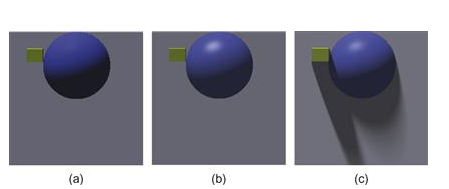
\includegraphics[width=\linewidth]{shading.png}
        \caption{Three types of shading}
    \end{figure}
    \begin{figure}[H]
        \centering
        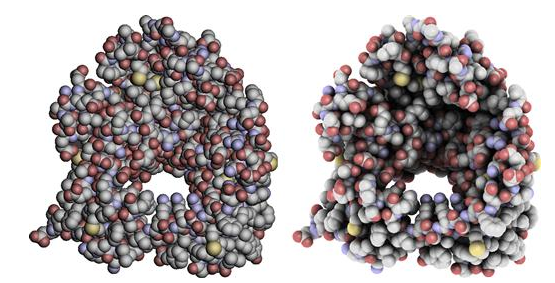
\includegraphics[width=\linewidth]{occlusion.png}
        \caption{Occlusion in a molecule visualization}
    \end{figure}

    \begin{figure}[H]
        \centering
        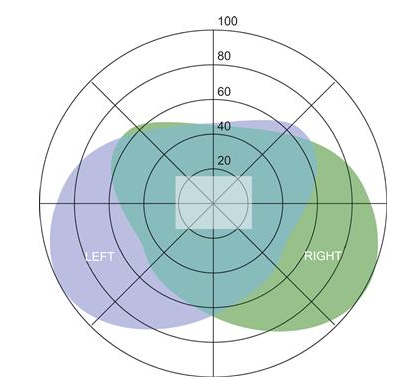
\includegraphics[width=0.6\linewidth]{visual_field.png}
        \caption{Visual field. Center square is a typical monitor}
    \end{figure}
\end{multicols}\end{mdframed}


\begin{mdframed}\begin{multicols}{2}
\subsection{The Eye}
    We do not see what is on the retina. The locus of conscious
    perception is higher up, with details lost.
\begin{compactdesc}
\item[Visual angle] angle subtended by an object at the eye of an observer.
    When 57cm away, 1cm is about 1 degree. Good apprx. for computer monitors.
\item[Lens] 59 diopters. Becomes less flexible with age. Lose about 2
    diopters per decade.
\item[Depth of Focus] At 50cm 43cm are near and 60cm are far. At 3m, 1.5m is
    near and $\infty$m is ``far''.
\item[Augmented reality] Superimpose visual imagery on the real world.
    Perspective is easy, eye position is difficult as is the design of
    optic systems to make light, undistorted and portable systems.
\item[Virtual reality] optical blur and optical distance must be simulated
    to accurately show depth. Eye tracker to determine the user's focus.
\item[Chromatic aberation] our eye is uncorrected for this. Blue on black is
    nearly indistinguishable. Can cause strong depth effects! Red on black
    seems nearer than blue on black for most people, though effect can be
    reversed.
\item[Retina] has two photoreceptor cells: rods (100 million) for low-light
    conditions, they are usually too stimulated to provide help and cones which
    are sensitive under normal levels (6 million).
\item[Fovea] center of the retina, densely packed only with cones. 2-degree
    field, best in the central $\frac{1}{2}$ degree.
\item[Simple acuities]:
    \begin{compactdesc}
    \item[Point (a)] acuity (1 minute of arc)
    \item[Grating (b)] acuity, bars (1 to 2 minutes of arc)
    \item[Letter (c)] acuity (5 minutes of arc). 20/20 vision means a 5 minute
        letter can be resolved 90\% of the time.
    \item[Stereo (d)] acuity, for depth (10 seconds of arc)
    \item[Vernier (e)] acuity, ability to see if two line segments are colinear
        (10 seconds of arc)
    \end{compactdesc}

\item[Binocular abilities] to perceive acuities improves by 7\% and
    contrast sensitivity increased by $\sqrt 2$.
\item[Acuity distribution] Only $\frac{1}{10}$ of detail 10 degrees from the
    fovea. Inverse square law.
\end{compactdesc}
\end{multicols}
\end{mdframed}


\begin{mdframed}\begin{multicols}{3}
    \begin{figure}[H]
        \centering
        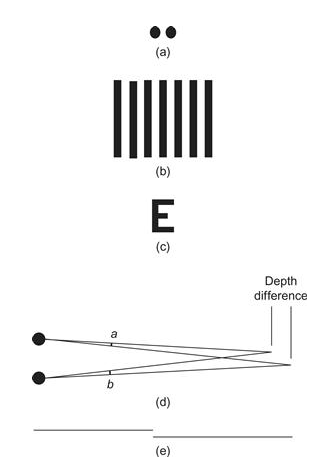
\includegraphics[width=0.7\linewidth]{acuities.png}
        \caption{Simple acuities}
    \end{figure}
    \begin{figure}[H]
        \centering
        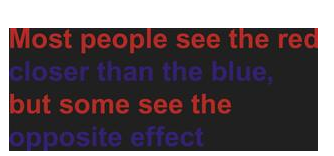
\includegraphics[width=\linewidth]{red_or_blue_near.png}
        \caption{Chromatic aberration}
    \end{figure}
    \begin{figure}[H]
        \centering
        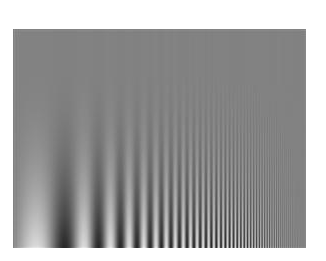
\includegraphics[width=\linewidth]{grating_gradient.png}
        \caption{Gradient along a grating pattern}
    \end{figure}

\end{multicols}\end{mdframed}




\begin{mdframed}
\begin{multicols}{2}
\begin{compactdesc}
\item[Axon] Thousands of photoreceptors (fewer in periphery) $\to$ ganglion
    cell, this is a type of neuron and it communicates using an axon. 3\% of
    the visual field receives half of the V1 neurons.
\item[Receptive field] area that feeds the retinal ganglion cells.
\item[Brain pixels] ganglion cells are the best match. Not uniformly
    distributed.
\item[Optimal screen]
    There are formulas for calculating efficiency of a
    screen. Though a typical monitor is only 5\% to 10\% of our visual field,
    it stimulates 50\% of our brain pixels. Small, high resolution with an
    interactive program beats low resolution and immersively large.
\item[Parafovea] best for pattern perception, 6 degrees, centered on fovea.
\item[Spatial contrast sensitivity] Most sensitive to dark bars on
    grey background at 2 to 3 cycles per degree. At age 80, less sensitive to
    $>1$ degree.
\item[Temporal contrast sensitivity] interdependent on spatial. Flicker. Most
    sensitive between 2 to 10 Hz.
\item[Visual stress] striped patterns of 3 cycles per degree, flicker at 20 Hz
    are the most likely culprits.
\item[Pattern-induced epilepsy] Avoid high contrast grating patterns or
    anything flickering at rates between 5 to 50 Hz.
\end{compactdesc}
\end{multicols}\end{mdframed}








\begin{mdframed}\begin{multicols}{2}
\subsection{The Optimal Display}
\begin{compactdesc}
\item[Dimensions] 4000 by 4000 pixels should be adequate. Printers use 1200
    dpi, this is to correct for the following two technical and one perception
    problem.
\item[Aliasing] mapping fine patterns to a pixel array causes errors. Our
    vernier acuity makes use sensitive to these problems. Fixed by computing
    a type of average of the input data, ``anti-aliasing. ''
\item[Number of dots] the 1200 dpi in a black and white printer are needed to
    print shades of gray. Aliasing effects are corrected by adding randomness
     to the dot position, instead of printing in square patches.
\item[Superacuities and displays] antialiasing enhances vernier acuity;
    even if the lines are subpixel size.
\item[Temporal requirements] our resolution limit is 50 Hz. Artifacts can be
    seen if the object moves too fast. Motion blur can fix.
\end{compactdesc}
\end{multicols}\end{mdframed}



 \section{Chapter 3: Lightness, Brightness, Contrast and Constancy}
\graphicspath{ {pngs/ch3/} }
%    \begin{figure}[H]
%        \centering
%        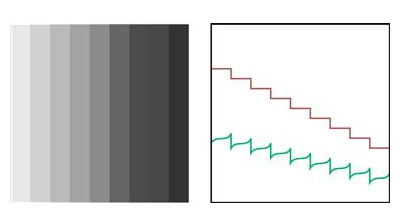
\includegraphics[width=0.4\textwidth]{chevreul_illusion.png}
%        \caption{Chevreul illusion, grayscale step patterns}
%    \end{figure}



\secttoc

    The eye detects changes in light on a surface, not absolute values. It is
    also nonlinear in this respect. Can cause errors, not good for categorical
    encoding. Very skilled at judging \emph{lightness}.
    Luminance is but one channel, but it its stronger than others, including
    color (b\&w films!).

\begin{mdframed}\begin{multicols}{2}

\subsection{Neurons, receptive fields and brightness illusions}
\begin{compactdesc}
    \item[Neurons] always firing, can be inhibited.
    \item[Layers of eye cells] \ce{->} retinal ganglion cells \ce{->} lateral
        geniculate nucleus \ce{->} V1.
    \item[Visual receptive field] the area over which a cell responds to light.
        On-center = active neurons, off-center = inhibited neurons. Modeled
        by DoG model (difference of Gaussians). Two exponential functions,
        $center - surround$. Edge receptors \emph{laterally inhibit} center
        receptors.
    \item{Hermann grid illusion} white intersections seem darker than the
        white bars between squares because they cause more inhibition.
    \item[Simultaneous brightness contrast] gray patch looks lighter
        on a dark background than on a light background. The DoG model
        shows significant difference in their (relative) brightness.
    \item[Mach bands] Bright band seen when uniform area meets a luminance
        ramp. (square gradient). DoG model predicts this.
    \item[Chevreul illusion] measured brightness = staircase, perceived =
        upticks as stairs.
    \item[Simultaneous contrast and errors] grayscale schemes can cause huge
        perception errors.
    \item[Edge enhancement] Lateral inhibition can be considered the first step
        of edge detection. Pseudo-edges can be created by having an
        edge between them that shades off gradually to two sides. Cornsweet
        effect. Clear inside/outside.
        \textbf{Haloing}.
\end{compactdesc}
\end{multicols}\end{mdframed}



\begin{mdframed}\begin{multicols}{2}
\subsection{Contrast effects and artifacts in Computer graphics}
Black on white is as distinctive as white on black. Only the difference
in luminance matters.
\begin{compactdesc}
    \item[Uniform shading] vertex uniformly colored based on facet's center's position.
        Chevreul illusion.
    \item[Gouraud shading] averages surface normals to shade edges of facets.
        Mach banding at boundaries.
    \item[Phong shading] Like Gouraud shading, but surface normal is
        interpolated between edges. No illusions, very smooth.
    \begin{figure}[H]
        \centering
        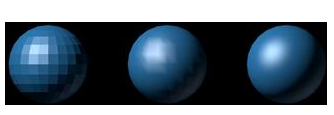
\includegraphics[width=0.3\textwidth]{shading.png}
        \caption{Illusions encountered in Uniform and Gouraud shading.}
    \end{figure}


\end{compactdesc}

\end{multicols}\end{mdframed}





\begin{mdframed}\begin{multicols}{2}
    \begin{figure}[H]
        \centering
        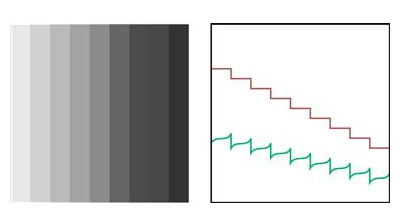
\includegraphics[width=0.3\textwidth]{chevreul_illusion.png}
        \caption{Chevreul illusion, grayscale step patterns}
    \end{figure}
    \begin{figure}[H]
        \centering
        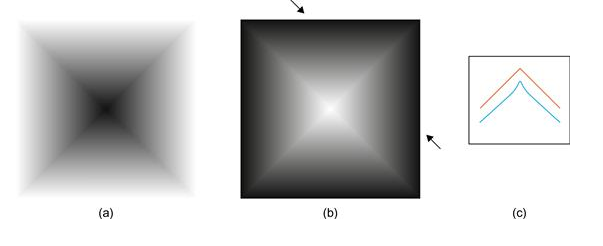
\includegraphics[width=0.3\textwidth]{mach_band_illusion.png}
        \caption{Mach band illusion. Rightmost panel is percevied lightness,
        calculated wiht DoG model.}
    \end{figure}
    \begin{figure}[H]
        \centering
        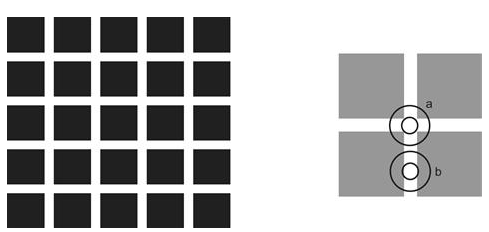
\includegraphics[width=0.3\textwidth]{hermann_grid_illusion.png}
        \caption{Hermann grid illusion. Inhibition may cause the artifacts in
        the grid intersections}
    \end{figure}
    \begin{figure}[H]
        \centering
        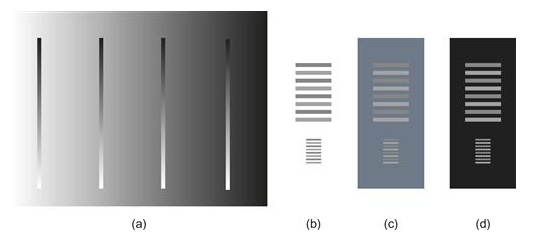
\includegraphics[width=0.3\textwidth]{contrast_crispening.png}
        \caption{Contrast crispening illusion}
    \end{figure}
\end{multicols}\end{mdframed}




\begin{mdframed}\begin{multicols}{2}
\subsection{Luminance, Brightness, Lightness and Gamma}
\begin{compactdesc}
    \item[Constancy] We must know about objects, not light itself. We
        experience colored surfaces, not colored light. Same for the
        overall reflectance of a surface. Black paper looks black under any
        magnitude of light.
    \item[Luminance] measured (real) amount of light
    \item[Brightness] perceived amount of light
    \item[Lightness] perceived reflectance of a surface, its
        gray-scale/saturation.

    \item[V$(\lambda)$ function] relates the sensitivity of the luminance
        channel to wavelength. We are about 100 times more sensitive to
        green light (550nm) than blue (450nm). Red is around 650 nm.
    \item[Finer details] require greater contrast. Minimum 3:1, text should be
        10:1. This limits available colors.
    \item[Brightness] perceived brightness (of a self-luminous source) is
        nonlinear related to the amount of light emitted by a lamp.
    \item[Sensation] $= aI^n$, intensity I. Also applies to other sensations:
        heaviness, smell, touch.
    \item[Monitor gamma] pixels emit nonlinear, gamma around 2.0 cancels a
        brightness power $n = 0.5$ to produce linear perceived brightness.
    \item[Lightness constancy] Help factor out the effects of amount and color
        of light. 1.\@ adaptation to available light. 2\@ lateral inhibition.
    \item[Huge range] amount of light in a dimly lit room is 10,000 times
        darker than that available on a bright day. \textbf{Photopigment} is
        bleached at high light levels, regenerates at lower levels.
    \item[Simultaneous contrast effect] can help us distinguish white from gray
        even though the two surfaces are on backgrounds of different luminance.
    \item[Contrast on paper and on screen] pictures are not just their image,
        but a surface as well! We perceive the actual gray levels of the
        photographic pigments, as opposed to the gray levels of what is depicted.
        Contrast illusions are stronger on computer displays. They are self
        luminous and there is no fine texture.
\end{compactdesc}
\end{multicols}\end{mdframed}

\begin{mdframed}
\begin{multicols}{2}
    \begin{figure}[H]
        \centering
        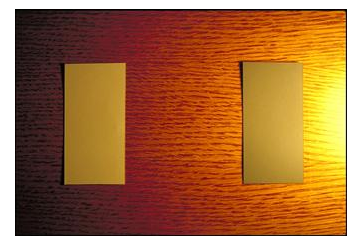
\includegraphics[width=0.7\linewidth]{lightness_constancy.png}
        \caption{Lightness constancy}
    \end{figure}


    \begin{figure}[H]
        \centering
        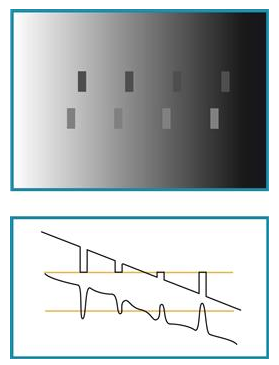
\includegraphics[width=0.4\linewidth]{simultaneous_brightness.png}
        \caption{Simultaneous contrast effect}
    \end{figure}
\end{multicols}\end{mdframed}


\begin{mdframed}
\subsection{Perception of surface lightness}
\begin{multicols}{2}
    The visual system can take into account the fact that a surface turned
    away from the light receives less light.



    We use the lightest object as a \textbf{reference white}.


    \textbf{Glossy highlights} matter. The most important thing separating an isolated
    black-world from a white-world is the ratio between specular and
    non-specular light.
\begin{compactdesc}
    \item[Uniform gray scale] bad, don't use. However, it illustrates some general
        issues related to perceptual scales.
    \item[Weber's law] For small differences in brightness, the value $\delta$
        in $\delta L$ is independent of the overall brightness. Screens
        only have 8 bit luminance, can't show.
    \item[Contrast crispening] Another distortion of gray values. Grays near
        similar gray backgrounds can be differentiated easier (crisper).

\end{compactdesc}
    \begin{figure}[H]
        \centering
        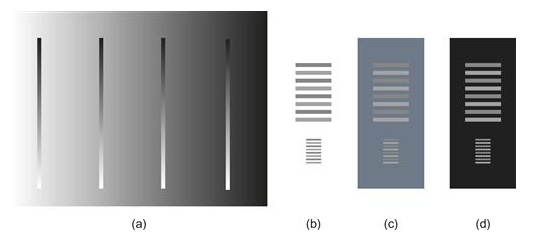
\includegraphics[width=0.3\textwidth]{contrast_crispening.png}
        \caption{Contrast crispening illusion}
    \end{figure}


\end{multicols}\end{mdframed}

\begin{mdframed}
\subsection{Monitor illumination and Monitor surrounds}
Important if accurate color display is needed, like fabric samples on
customer's screen, or for an artist's screen. How to setup lightning around
monitor?
\begin{compactdesc}
    \item[Ambient room illumination,] keep screen emission and room ambience
        at similar luminance. (Normal: 5\% to 20\% of screen light is just
        reflected from room). Really bad with white projector screens.
    \item{Contrast reduced} when room light falls on display.
        $L_{monitor} = V^r + A$ where A is ambient illumination, V
        is voltage, L is luminance output for a given gamma.
    \item{Equal voltage steps} \textbf{= equal perceptual steps}, a lower
        gamma is needed. Dark viewing conditions = higher gamma.
    \item{Room} should have a standard light level and illuminant color.
        The white of the monitor should match the white of a paper help up by
        screen.
\end{compactdesc}

\begin{multicols}{2}

\end{multicols}\end{mdframed}

 \section{Chapter 4: Color}
\graphicspath{ {pngs/ch4/} }


\secttoc

Although color is the most studied feature of perception, the results are few.
Most important is opponent process theory.
This discussion continues in other chapters.

\begin{mdframed}\begin{multicols}{2}
\subsection{Trichromacy theory}
Color vision helped break camouflage. Color is more of an attribute than a
primary characteristic.
Chickens have 12 kinds of color-sensitive cells.
\begin{compactdesc}
    \item[Color] excellent for labeling or categorization. We have 3 kinds
        of color-sensitive cells. These three  colors can be mixed together
        to simulate other colors.
    \item[Cones]
        Rods are overstimulated at most light levels and rendered useless.
    \item[Color blindness] 10\% male, 1\% female. Most common is the lack of
        long-wavelength (protanopia) or medium-wavelength (deuternopia).
        Respectively, can't see red or green. 3D space collapses to 2D space.
\end{compactdesc}
    \begin{figure}[H]
        \centering
        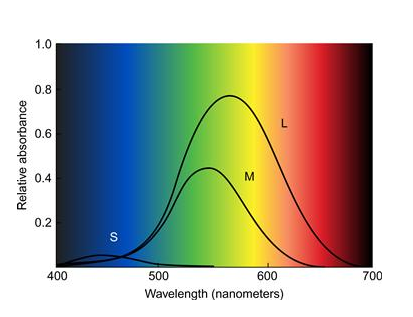
\includegraphics[width=0.4\textwidth]{cone_sensitivity.png}
        \caption{Cone sensitivity functions}
    \end{figure}


\end{multicols}\end{mdframed}


\begin{mdframed}\begin{multicols}{2}
\subsection{Color measurement}
\begin{compactdesc}
    \item[CIE tristimulus system] is the most precise, closest to our perceptive
        abilities.
    \item[CIElab and CIEluv] are examples of equidistant color spaces.
        The same offsets produce the same color differences, unlike in the
        CIE space.
    \item[Useful] but even the equidistant spaces cannot be used to predict
        how a color will be perceived. Thin lines? Hard to distinguish
        along the yellow-blue.

    \item[Gamut] 3D figure representing color perception ability in terms
        of red, green and blue.
    \item[Primaries] can be mixed to produce any color
    \item[Purple boundary] connecting red (700nm) to blue (400nm).
\end{compactdesc}
    \begin{figure}[H]
        \centering
        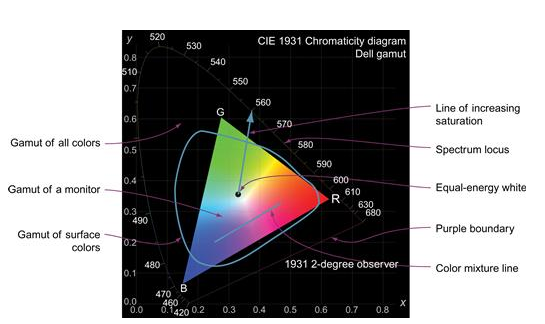
\includegraphics[width=0.4\textwidth]{cie_chromaticity.png}
        \caption{The CIE chromaticity diagram (interesting features)}
    \end{figure}


\end{multicols}\end{mdframed}


\begin{mdframed}\begin{multicols}{2}
\subsection{Opponent Process Theory}
\begin{compactdesc}
    \item[Opponent-pairs] Cornerstone of modern color theory.
        Black-white, yellow-blue and red-green lie on the same axis.
    \item[Naming] impossible: reddish green, yellowish blue. Confirmed.
    \item[Cross-cultural naming] 100 languages! Primary color terms are
        consistent, first are black and white. Next is red. The fourth and
        fifth are always yellow or green. The sixth is always blue. Seventh is
        brown followed by pink, purple, orange, and gray in no order.
    \item[Unique hues] we can identify yellow to 2nm. Green is either at 514nm
        or 525nm (for $\frac{1}{3}$ of population). Mostly independent of
        luminance level.
    \item[Neurophysiology] Cells in primary visual cortexes of monkeys have the
        properties predicted by opponent process theory.
    \item[Categorical colors] colors close to the ideal primaries are easy to
        remember. Colors that are not basic, like orange or lime  green are
        difficult to remember. Only eight colors and white were accurately named.
\end{compactdesc}
\end{multicols}\end{mdframed}


\begin{mdframed}\begin{multicols}{2}
\subsection{Properties of color channels}
\begin{figure}[H]
\centering
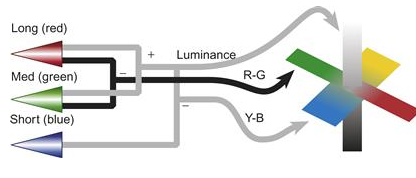
\includegraphics[width=0.4\textwidth]{opponents.png}
\caption{Opponent colors}
\end{figure}

\begin{figure}[H]
\centering
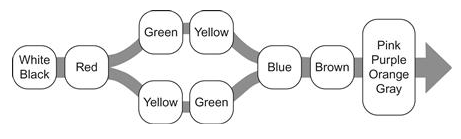
\includegraphics[width=0.4\textwidth]{color_order.png}
\caption{Cross cultural color order}
\end{figure}
\begin{figure}[H]
\centering
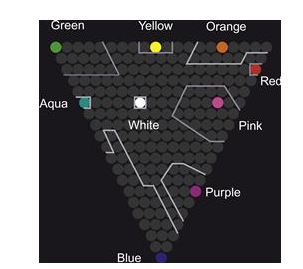
\includegraphics[width=0.6\linewidth]{accurately_identified.png}
\caption{8 colors identified 75\% of the time}
\end{figure}



\end{multicols}\end{mdframed}


\begin{mdframed}\begin{multicols}{2}
\subsection{Properties of color channels}
\begin{compactdesc}
    \item[Isoluminant/equiluminous] same grayscale. Stereo depth i
    \item[Spatial sensitivity] the two chromatic colors carry only one-third
         of the information that the grayscale does. Chromatic differences are
         not suited for displaying any kind of detail.
    \item[Stereoscopic depth] only detected using luminance.
    \item[Motion sensitivity] easier to see the motion of objects with
        different luminance, colored looks slower.
    \item[Form] we're very good at perceiving shapes; but if chromatic
        differences are used for textures, expect weaker looking surfaces.
    \item[Summary] red-green, yellow-blue inferior in most respects to
        luminance
\end{compactdesc}
\end{multicols}\end{mdframed}


\begin{mdframed}\begin{multicols}{2}
\subsection{Color appearance}
\begin{compactdesc}
    \item[Monitor surrounds] it is important to pay attention to the environment
        of a monitor, for it affects colors perceived.
    \item[Color constancy] we cannot see absolute colors, they depend entirely
        on surrounding colors. Tungsten light is much more yellower than
        sunlight, but this is not often noticed.
    \item[Color contrast] similar to lightness contrast (chapter 3), can
        distort readings of a color-coded map. Relative color is much more
        important than absolute color.
    \item[Saturation] high: far from the grayscale, low: dull or grayish.
        Few saturation steps can be accurately distinguished.
    \item[Brown] wtf. Dark yellow, but rarely referred to this way. People may
        need a reference white to see it. May not be distinguishable in a set
        of color codes.
\end{compactdesc}
\begin{figure}[H]
\centering
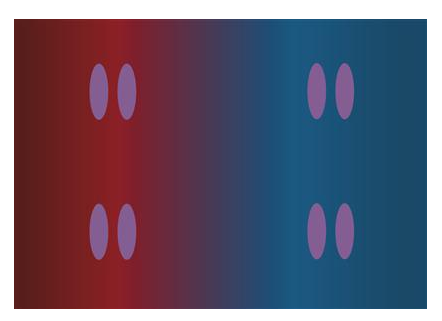
\includegraphics[width=0.4\linewidth]{color_contrast.png}
\caption{Color contrast illusion}
\end{figure}


\end{multicols}\end{mdframed}


\begin{mdframed}\begin{multicols}{2}
\subsection{App 1: Color specification interfaces}
\begin{compactdesc}
    \item[Color spaces] design a color picker! Best to offer a method showing
        colors on different backgrounds.
    \item[HSV] hue, value and saturation.
    \item[RGB] red, green and blue.
    \item[Color naming] People agree on few names. There exist large maps
        from intuitive names to actual values: NCS, Pantone (USA printing),
        Munsell (USA surfaces).
    \item[Color palettes] should provide ability to create personalized
        palettes.
\end{compactdesc}
\end{multicols}\end{mdframed}


\begin{mdframed}\begin{multicols}{2}
    \subsection{App 2: Color for labeling (nomial codes)}
    Perceptual factors to consider when picking a set of color labels.
\begin{compactdesc}
\item[Distinctness] uniform (equidistant) color space can be used to determine
    the difference between two colors. Must also consider background and area.
    \item[Unique hues] Red, green, yellow, blue, as well as black and white.
        Small set of color codes required.
    \item[Contrast with background] should consider different backgrounds.
        Always make sure there is a luminance difference if symbols must be
        distinguished from background.
    \item[Color blindness] Yellow-blue direction is most universal.
    \item[Number] Five to ten elements can fit in a color code.
    \item[Field size] Do not use very small color-coded areas. Yellow-blue is
        hard to distinguish at small sizes.
    \item[Conventions] Pay attention. Domain specific. Example: hot = red,
        cold = blue.
\end{compactdesc}
\begin{figure}[H]
\centering
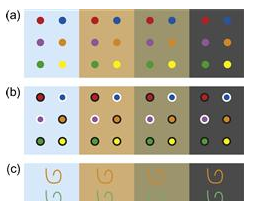
\includegraphics[width=0.4\textwidth]{colors_on_backgrounds.png}
\caption{Colors on different backgrounds. Lines especially difficult}
\end{figure}



\end{multicols}\end{mdframed}


\begin{mdframed}\begin{multicols}{2}
\subsection{App 3: Color sequences for data maps}
\begin{compactdesc}
    \item[Chloropleth map] representing continuous values on a map using color
    \item[Form and quantity] Different color sequences have different effects
        when used for ranking. Can be actively misleading. Best to use
        a straight line through a uniform color space. Could use a spiral
        sequence.
    \item[Interval pseudocolor sequences] contours and a discrete sequence
        of colors (not smooth) work well.
    \item[Ratio pseudocolors] if values are signed, such a sequence is called
        diverging or bipolar.
    \item[Sequences for the color blind] There are specially designed color
        sequences.
    \item[Bivariate color sequences] hue and lightness/saturation works well.
        Don't use color on two axes, they end up unreadable.
    \item[Best of the best] let a user with enough time decide what shows
        the most information for them.
\end{compactdesc}
\end{multicols}\end{mdframed}


\begin{mdframed}\begin{multicols}{2}
\subsection{App 4: Color reproduction}
    Most output devices cannot reproduce the 16 million colors that can be
    created by a monitor.


    Good mapping from one device to another:
\begin{compactenum}
    \item White should look white on both devices, same goes for black
    \item Maximum luminance contrast is desirable
    \item Few colors should lie outside target gamut
    \item Hue/saturation shifts should be minimized
    \item Increase in saturation is preferable to a decrease
\end{compactenum}
\begin{compactdesc}
    \item[Calibration] setup a common reference
    \item[Range scaling] scale about the luminance axis
    \item[Rotation] find the neutral white. The two white axes should coalign.
    \item[Saturation scaling] Scale radially.
    \item[Modern printers] use heuristics, though an educated technician can do
        better.
\end{compactdesc}
\end{multicols}\end{mdframed}




 \section{Chapter 5: Visual salience and finding information}
\graphicspath{ {pngs/ch5/} }
%    \begin{figure}[H]
%        \centering
%        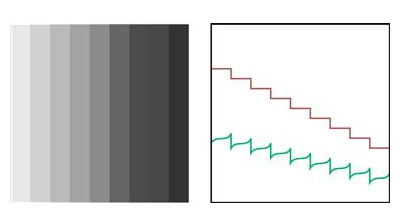
\includegraphics[width=0.4\textwidth]{chevreul_illusion.png}
%        \caption{Chevreul illusion, grayscale step patterns}
%    \end{figure}


\secttoc

\textbf{Symbol} is an object representing an entity.
\textbf{Glyph} is a symbol meant to convey one or more numerical attributes
of that entity.
We mostly see what we expect to see.
Glyphs must stand out in at least one channel.
For low-level properties, like interferes with like.
Channels can be separable or holistic.
Must make fundamental design choices and tradeoffs.

\begin{mdframed}\begin{multicols}{2}
\subsection{Eye movements}
\begin{compactdesc}
    \item[Saccades] a fast change of focus. 2-5 per second while reading.
        Said to be \emph{ballistic}, they cannot be adjusted mid-movement.
    \item[Saccadic suppression] During such a movement, we are less sensitive
        to visual input.
    \item[Saccadic movements] Rapid movement between fixations.
        Dwell period between 200 and 400 msec.
        Saccade takes 20 to 180 msec, depends on angle. 2 degrees while
        reading. 2 to 5 degrees is good.
    \item[Smooth-pursuit movements] eye can pursue smooth moving objects. Can
        also make head/body movements to follow.
    \item[Convergent movements] Also called vergence movements. When an object moves
        towards us, eyes converge. Moves away, eyes diverge. Can be either
        saccadic or smooth.
    \item[Accomodation] refocusing takes about 200 msec. Ability declines with
        age, fix with different-lens glasses or laser surgery (one near, one
        far).
\end{compactdesc}

\subsubsection{What is easily findable?}
How do we know where to look next? Heuristics strategy: focus on features that
fit our goal most closely.
\begin{compactdesc}
    \item[A priori salience] some patterns excite more neural activity than
        others.
    \item[Top-down salience modification] Depends on our goal. We can focus on
        relevant low-level V1 features.
    \item[Scene gist] Less about feature maps, more experience. Eye movements
        can be primed to specific types of learned scenes.
\end{compactdesc}
\end{multicols}\end{mdframed}



\begin{mdframed}\begin{multicols}{2}
    \begin{figure}[H]
        \centering
        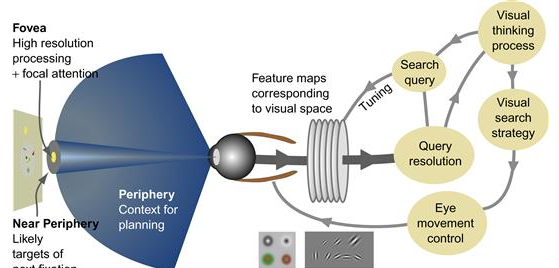
\includegraphics[width=\linewidth]{visual_search.png}
        \caption{The process of visual search}
    \end{figure}
    \begin{figure}[H]
        \centering
        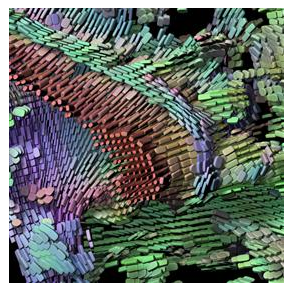
\includegraphics[width=0.6\linewidth]{tensor_vis.png}
        \caption{3D tensor field visualization using color, orientation and
        shape.}
    \end{figure}


\end{multicols}\end{mdframed}


\begin{mdframed}\begin{multicols}{2}
\subsection{V1, Channels, and Tuned Receptors}
\begin{compactdesc}
    \item[V1 and V2] V1 passes mostly to V2, they represent 40\% of vision
        processing. Several billion neurons devoted to analyzing output from
        several million nerve fibers.
    \item[Optic nerves] split the image into red-green, yellow-blue and
        dark-light channels before sending to V1.
    \item[Semi-independent features] processed by V1, V2:
        \begin{compactenum}
        \item Orientation and size (with luminance)
        \item Color via opponent processing
        \item Elements of local stereoscopic depth
        \item Elements of local motion
        \end{compactenum}
        A feature close to another feature is processed by nearby neurons.
    \item[Elements of form] These features are like phonemes in speech.
        Can be independent of each other. Color, form and motion.
        More complex composite patterns aren't processed as rapidly.
    \item[Assumption:] single neurons can be treated as independent.
        Groups of neurons or synchronization or temporal spacing also encode
        information, maybe more?
    \item[V1 and V2] continually process orientation and size. Each of the stages
        has a preferred size/orientation.
    \item[Gabor model and visual distinctness] Simple mathematical model:
        multiply a cosine wave by a Gaussian envelope. Excitory center flanked
        by two inhibitory bars. Variables: amplitude/contrast, size, and
        rotation. Detect particular orientations but not right-angles.
    \item[Barlow's 2nd dogma] fits with Gabor model. Simultaneously optimized
        for spatial location, size and orientation.
    \item[Gabor detectors] process image in terms of spatial frequency channels.
        Sub-channels of texture and elements of shape. Orientation sensitivity:
        30 degrees. Size: 2x.
    \item[Fine discrimination] when given more time, people can resolve far
        smaller differences than with brief exposures. Size: 9\%, orientation:
        5 degrees.
        Higher level processes sharpen the output from individual neurons.
        Common. Operates by comparing \emph{differences} between many neurons.
    \item[Point:] use size differences, color and orientation to differentiate
        symbols.
\end{compactdesc}
    \begin{figure}[H]
        \centering
        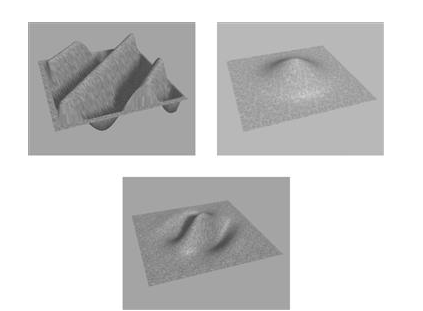
\includegraphics[width=0.5\linewidth]{gabor.png}
        \caption{Gabor detector, a sine wave multiplied by a Gaussian envelope}
    \end{figure}

\end{multicols}
\end{mdframed}



\begin{mdframed}\begin{multicols}{2}
\subsection{Pre-attentive processing and ease of search}
\begin{compactdesc}
    \item[Preattentive processing] captures certain features, entities
        ``pop out.'' Such features can be detected despite distractors.
        Misleading name, attention and perception are tightly bound.
        Anything processed faster than 10 msec. Others are $>$ 40 msec.
    \item[Features] categorized into form, color, motion, and spatial
        position:
        \begin{compactenum}
        \item Line orientation
        \item Line length, width
        \item Size
        \item Curvature
        \item Spatial grouping
        \item Blur
        \item ``Added marks''
        \item Numerosity
        \item Color, hue, intensity
        \item Motion, direction of
        \item Flicker
        \item Direction of motion
        \item Spatial position
        \item 2D position
        \item Stereoscopic depth
        \item Convex/concave from shading
        \end{compactenum}
    \item[Attention and expectation] subjects can ignore features if unexpected.
    \item[Highlight] an object by granting it a positively asymmetric
        pre-attentive cues, such as color in a black and white field.
        Subtle motion in static display.
    \item[Redundant features] can be used for more effective searches.
    \item[Not easily findable:] conjunction of features. For example: find the
        red square. Some exceptions:
        \begin{compactenum}
        \item spatial grouping on XY plane
        \item stereoscopic depth and color or movement
        \item luminance polarity (white on grey) and shape
        \item Convexity/concavity and color
        \item Motion and anything
        \end{compactenum}
\end{compactdesc}
\end{multicols}
\end{mdframed}



\begin{mdframed}\begin{multicols}{2}
    \begin{figure}[H]
        \centering
        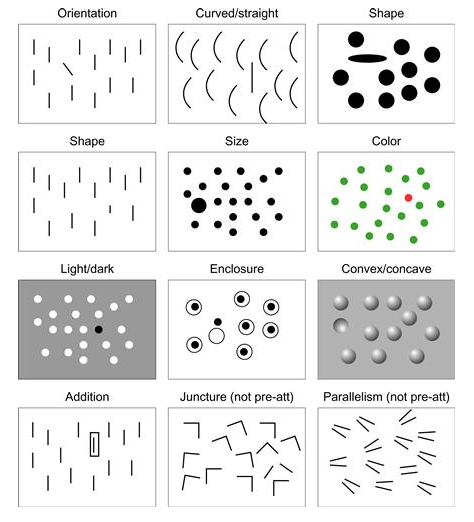
\includegraphics[width=0.25\textwidth]{preattentive.png}
        \caption{Array of preattentively processed features}
    \end{figure}


    \begin{figure}[H]
        \centering
        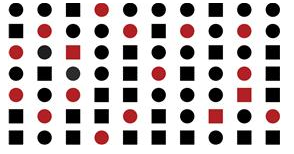
\includegraphics[width=0.3\textwidth]{find_red_square.png}
        \caption{Find the red square}
    \end{figure}

\end{multicols}
\end{mdframed}



\begin{mdframed}\begin{multicols}{2}
\subsection{Integral and separable dimensions. Glyph design.}

    \begin{figure}[H]
        \centering
        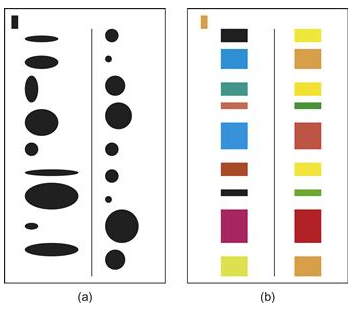
\includegraphics[width=0.5\linewidth]{speeded_classification.png}
        \caption{Speeded classification experiments. On height. In (a) the
        variable width interferes with classification. In (b) the variable
        color does not interfere}
    \end{figure}
\begin{compactdesc}
    \item[Garner's theory:] there are integral and separable dimensions.
    \item[Glyph] symbols representing quantity
    \item[Questions answered:]
        ``Will the color-scheme interfere with glyph size?''
        ``Will using both color and size make a variable clearer?''
        Will displays be perceived independently from each other?
    \item[Integral display dimensions] two attributes are perceived
        holistically and not independently
    \item[Separable dimensions] separate judgments can be made about
        each graphical dimension.
\end{compactdesc}
    \begin{figure}[H]
        \centering
        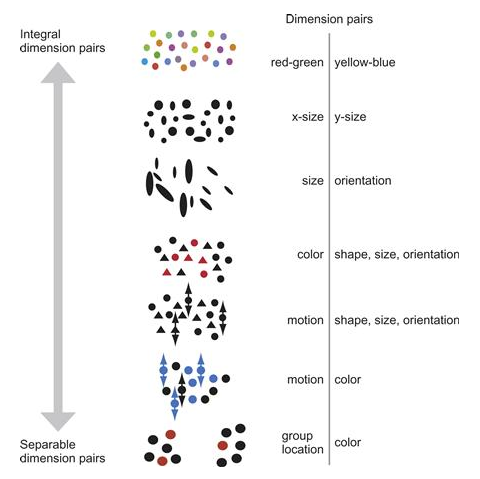
\includegraphics[width=0.5\textwidth]{integral_separable.png}
        \caption{Integral and separable dimension pairs}
    \end{figure}

\end{multicols}
\end{mdframed}



\begin{mdframed}\begin{multicols}{2}
\subsection{Representing quantity}
\begin{compactdesc}
    \item[Monotonic visual qualities] increase continuously: size,
        brightness, height. Cyclic: angle, phase of motion, hue.
    \item[Ranking] height $>$ area $>$ 3D volume $>$ grayscale.
        Area can convey greater variations.
    \item[Exact quantities] numerical annotation, bar graph, wind barb (can
        encode 30 steps, but distort wind direction).
    \item[Multidimensional discrete data]
        These are the most useful attributes in glyph design
    \begin{compactdesc}
        \item[Spatial position] 3 dimensions, XYZ
        \item[Color] 3 dimensions, color opponent theory
        \item[Shape] ?, size, orientation are basic, may be more, dimensions are
            certainly small
        \item[Surface texture] 3 dimensions, orientation size and contrast.
        \item[Motion coding] 2-3 dimensions, phase is critical, more research
            needed
        \item[Blink coding] 1 dimension, interdependent with motion
    \end{compactdesc}
        Number of resolvable steps is small. Conjunctions are not generally
        pre-attentive, unfortunately limiting us to about 32 distinct glyphs.
    \item[Stars and whiskers]
        No natural mappings to channels? Use whisker/star plots. Each variable
        is a line emanating from the center. Four whiskers is probably the
        maximum. Use parallel coordinates in case of multiple data.
    \begin{figure}[H]
        \centering
        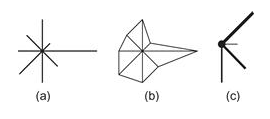
\includegraphics[width=0.2\textwidth]{whisker_star.png}
        \caption{(a) whisker plot, (b) star plot, (c) whisker with four variables and varying width}
    \end{figure}
\end{compactdesc}
\end{multicols}
\end{mdframed}


\begin{mdframed}\begin{multicols}{2}
\subsection{Searchlight metaphor and cortical magnification}
\begin{compactdesc}
    \item[Searchlight] consider the eyeball as an information-gatherer.
        Information comes in bursts, snapshot for each fixation. Nonpreattentive
        objects arrive at 40 items per second.
    \item[Useful field of view] we can quickly take information from here.
        Varies greatly, from 1 to 4 degrees of visual angle for densely
        populated targets. Can be as large as 15 degrees.
    \item[Tunnel vision] the UFOV can be extremely compressed under large
        cognitive load. Consider this when designing user interrupts.
    \item[Role of motion in attention] UFOV is larger when detecting moving
        targets. UFOV around 40 degrees.
    \item[User interrupts]
        \begin{compactenum}
        \item easily perceived, even outside of fovea
        \item can be ignored, serve as reminder
        \item non irritating
        \item can be endowed with varying levels of urgency
        \end{compactenum}
    \item[Motion as a user interrupt]
        Ship alarm flash patterns: subjects ID'd five patterns with 98\%
        reliability. Motion/blinking are reliable, but can be annoying.
        Slow motion need not be.
\end{compactdesc}
\end{multicols}
\end{mdframed}





 \section{Chapter 6: Static and Moving Patterns}
\graphicspath{ {pngs/ch6/} }

\secttoc

What is the best mapping from structured data to the display?
How can 2D space be divided into perceptually distinct regions?
Under what conditions are patterns perceived similar?
Visual connection between objects?
Mostly 2D, although some 3D properties are also important.
Pattern finding, hooray!


Visual system ranges from massively parallel primitive processing to high level
analysis of about one to five objects per fixation. Pattern perception is the
middle ground.


\begin{mdframed}\begin{multicols}{2}
    \subsection{Gestalt (pattern in German) Laws}
    A group of German psychologists in 1912 founded the Gestalt school of
    psychology.


    \begin{compactdesc}
        \item[Proximity] perceptual organization. Small spacing can have large
            effects. Consider spatial concentration and small size of fovea.
        \item[Similarity] similar elements should be grouped. Use channel theory
            and integral/separable dimensions. Good for independent patterns.
        \item[Connectedness] overlooked by originals. Connecting by lines.
        \item[Continuity] Smooth continuous objects are perceived better.
        \item[Symmetry] so good! Maybe for two time series? Important patterns
            must be small. 1 degree in width, 2 degrees in height centered at
            fovea. Don't make it too large. Horizontal/vertical is easier to
            see. Provide a frame of reference.
        \item[Closure and common region] Closed contours are seen as objects.
            Open ones are broken. Great for inside-outside divisions.
            Venn-Euler diagrams are used during introduction to set theory.
            Also used in window-based computer UIs.
        \item[Clarify closures] if they have a complicated shape with
            a Cornsweet edge, texture or color.
        \item[Figure-ground] figure is perceived in the foreground.
            Ground is everything ``behind'' it. Many Gestalt features help
            people segment (or not) an image. Closed contour, symmetry,
            amount of white area all contribute.
        \item[Relative size] smaller things are more object-like.
        \item[Rubin's Vase figure] high-level learned face recognition fights
            mid-level Gestalt figure detection processes.
        \item[Common fate] a motion based law discussed later.
        \item[More on Contours] continuous elongated boundaries between
            regions. Fundamental, receives much attention.
        \item[Randomly placed and oriented] Gabor patches. Continuity
            between patches with linear continuity is easiest to perceive.
            More wiggly patterns can also be detected.
        \item[Theory] inhibition between neurons with nonaligned receptive
            fields and mutual reinforcement between neurons with smoothly
            aligned patches. The winner take-all effect!
        \item[Controversial synchronous firing theory] neurons firing united
            may be how the brain retains higher-level patterns.
            Even if false, there is some neural mechanism enhancing contour
            detection.
    \end{compactdesc}
    \begin{figure}[H]
        \centering
        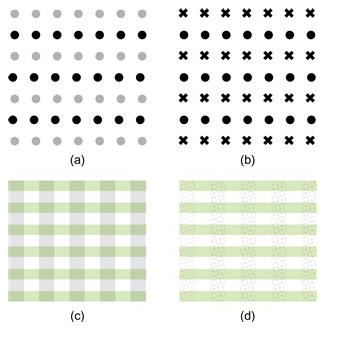
\includegraphics[width=0.2\textwidth]{Gestalten/similarity.png}
        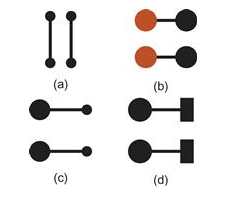
\includegraphics[width=0.2\textwidth]{Gestalten/connectedness.png}
        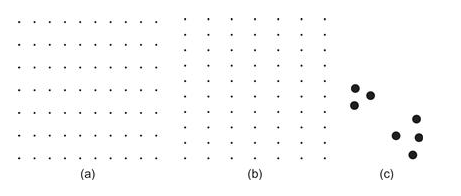
\includegraphics[width=0.2\textwidth]{Gestalten/proximity.png}
        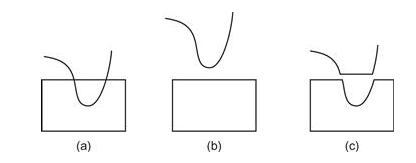
\includegraphics[width=0.2\textwidth]{Gestalten/continuity.png}
        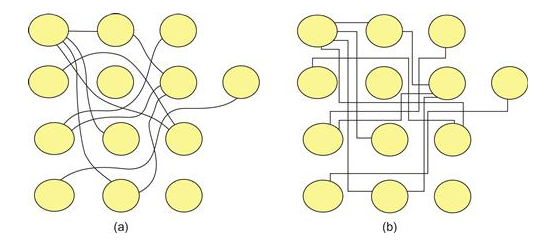
\includegraphics[width=0.2\textwidth]{Gestalten/continuity2.png}
        \caption{Similarity, connectedness, proximity, and continuity$\cdot2$}
    \end{figure}
    \begin{figure}[H]
        \centering
        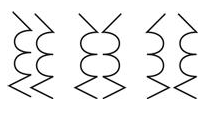
\includegraphics[width=0.1\textwidth]{Gestalten/symmetry.png}
        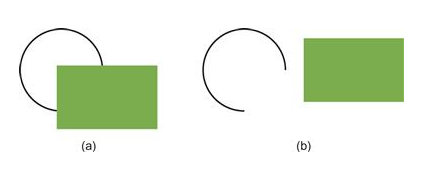
\includegraphics[width=0.15\textwidth]{Gestalten/closure.png}
        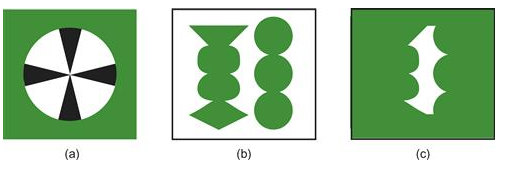
\includegraphics[width=0.15\textwidth]{Gestalten/figure_ground.png}
        \caption{Symmetry, closure, and figure and ground}
    \end{figure}
\end{multicols}\end{mdframed}

\begin{mdframed}
\begin{multicols}{2}
    \begin{figure}[H]
        \centering
        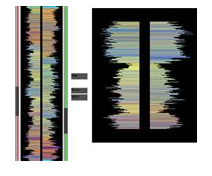
\includegraphics[width=0.4\textwidth]{symmetry_vis.png}
        \caption{Vis showing similarity in two time series using symmetry.}
    \end{figure}
    \begin{figure}[H]
        \centering
        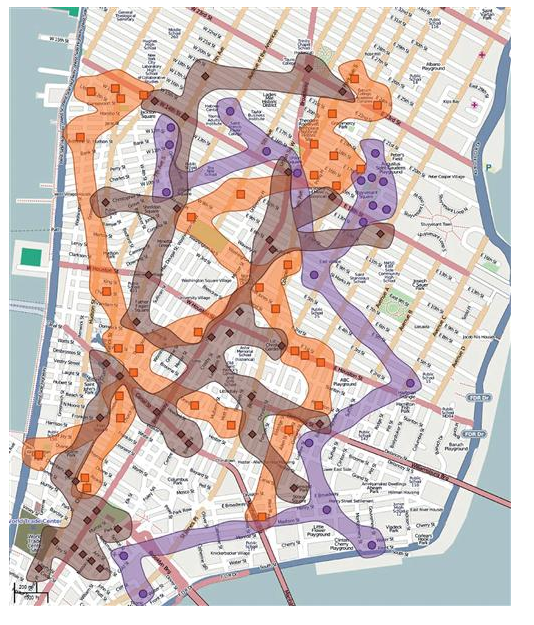
\includegraphics[width=0.3\textwidth]{color_and_region_vis.png}
        \caption{Contour, color and transparency to show distribution of
            hotels (orange), subway stations (brown), and medical clinic
            (purple).}
    \end{figure}
\end{multicols}
\end{mdframed}


\begin{mdframed}\begin{multicols}{2}
\subsection{Visualizing Vector Fields}
\begin{compactdesc}
    \item[Perceiving Orientation and direction] and magnitude.
    \item[Comparing 2D Flow Visualization techniques]
        A head to tail arrangement of vectors is ideal. Continuous contours
        provide the easiest perception of orientation, but do not show
        direction or magnitude. Randomly spaced, unconnected vectors are no
        good.
    \item[Tasks during flow visualization] are varied and depend on the
        application. Here are some:
        \begin{compactenum}
        \item Speed, orientation and direction at an arbitrary point
        \item Location and nature of critical points
        \item Advection trajectory
        \item High and low magnitude
        \item High and low curl
        \item High and low turbulence
        \end{compactenum}

    \item[Showing direction]
        Plain arrows produce clutter with their contours, their directional
        asymmetry
        is weak.
        It is better to use long narrow airfoils/pen-strokes.
        Can also vary gray level along the arrow. Called ``streamlets.''
        Stronger neural signal = more magnitude.

\end{compactdesc}
    \begin{figure}[H]
        \centering
        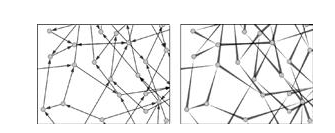
\includegraphics[width=0.25\textwidth]{link_vis.png}
        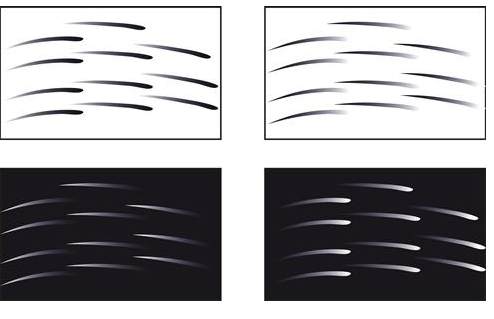
\includegraphics[width=0.2\textwidth]{streamlets.png}
        \caption{Left: two methods of drawing links, middle is more effective.
        Right: streamlets, effective for links}
    \end{figure}
    \begin{figure}[H]
        \centering
        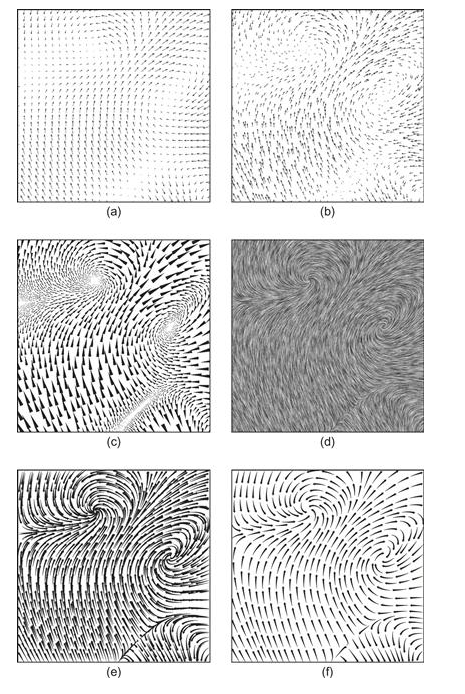
\includegraphics[width=0.6\linewidth]{six_flows.png}
        \caption{Six different vector field visualizations.
        Arrows a regular grid, arrows on a jittered
        grid to reduce perceptual aliasing, triangle icons with size
        indicating strength (density inversely related to size), line
        integral convolution, large-head arrows along a stream-line instead of
        a grid, large-head arrows along streamlines with constant spacing.}
    \end{figure}
\end{multicols}\end{mdframed}

\begin{mdframed}\begin{multicols}{2}
\subsection{Texture: Theory and Data Mapping}
    \begin{figure}[H]
        \centering
        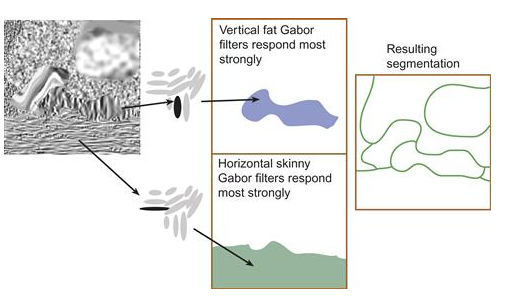
\includegraphics[width=\linewidth]{gabor_and_texture.png}
        \caption{Gabors can explain texture-based segmentation}
    \end{figure}

\begin{compactdesc}
    \item[Texture segmentation] regions defined by texture. Independent axis.
    \item[Gabor] is a Gaussian envelope * sine wave
    \item[Gabor filters] respond strongly to areas with dominant spatial
        frequencies and orientations. Contrast of textures is an independent
        feature.
    \item[Feature map] consisting of Gabors of different orientation can show
        primal sensitivity.
\end{compactdesc}

    \begin{figure}[H]
        \centering
        \includegraphics[width=0.7\linewidth]{gabors_and_classification.png}
        \caption{(a) Ts and Ls are difficult to segment, but the leaning Ts can
        be distinguished easily. (b) feature map of vertical gabors. (c)
        feature map of oblique gabors}
    \end{figure}

\end{multicols}\end{mdframed}



\begin{mdframed}\begin{multicols}{2}
\subsection{Information Density, An Uncertainty Principle}
\begin{compactdesc}
    \item[Perception of position, orientation, and size] are related
        by an uncertainty principle.
    \item[Orientation] can't use size as much
    \item[Size] less detail can be shown with larger elements
    \item[Gabors] can be stretched to specify either spatial frequency (size)
        or orientation more precisely.
    \item[Primary dimensions of texture]
        Real Gabors expose many variables, but in our visual systems Gabors
        with large Gaussians are coupled with high frequency cosine components
        and same goes for small and low frequencies. Thus a simpler three
        component model can be proposed:
        \\
        Orientation: cosine component
        \\
        Scale: $\frac{1}{spatial freq}$
        \\
        Contrast: Amplitude or contrast
    \item[Texture contrast effect] the same texture overlayed on another
        appears different. Some textures can interfere with other components,
        like lines.
    \item[Other dimensions] the world of texture is much richer than these
        three variables, though they are dominant. Randomness is also
        important.
    \item[Nominal coding] is the most common use for textures.
        Spatial frequencies should differ by a factor of 3, orientation
        by 30 degrees; where all other primitive factors are held constant.
\end{compactdesc}
    \begin{figure}[H]
        \centering
        \includegraphics[width=0.4\textwidth]{texture_contrast.png}
        \caption{The texture contrast effect. The two patches on the left and
            right have the same granularity, but the texture contrast makes
            them seem different.}
    \end{figure}
\end{multicols}\end{mdframed}



\begin{mdframed}\begin{multicols}{2}
\subsubsection{Case studies and more texture}
\begin{compactdesc}
    \item[Univariate and multivariate Maps] Scalars: most common is to
        vary element size according to the value. Limited because
        elements must be small to accommodate the data.
    \item[Orientes sliver textures] for more than one scalar.
        Sliver contrast indicates magnitude, each dimension has its own sliver
        orientation. Not readable with many variables.
    \item[Attempt two:] glyph color (temperature), orientation and direction
        (wind), glyph area coverage (wind speed), density of elements
        (pressure).
    \item[3, a Scientist and designer:] cross-section of a mouse spinal column.
        Shows 7 variables at each location. Tradeoffs. Glyphs are textured,
        and end up camouflaged. Worsened by texture orientation.
        Luminance has the highest range, all other components cause noise and
        distract from detail.
    \item[Quantitative texture sequence 1] 10-step texture steps and color.
        Textures gain luminance. Two maps are successfully combined.
    \item[Quantitative texture sequence 2] 14-step texture (different shapes,
        contrast) steps, color, animated streamlet vector field, number labels
        and a map of the Northwestern USA.
        Amen! Will need training.
    \item[Texture is most valuable] if there are two scalar values.
        To be reasonable, it consumes some luminance channel.
\end{compactdesc}
\end{multicols}\end{mdframed}

\begin{mdframed}\begin{multicols}{4}
    \begin{figure}[H]
        \centering
        \includegraphics[width=0.2\textwidth]{color_and_texture_vis.png}
        \caption{Bivariate map, color and a carefully designed texture sequence}
    \end{figure}
    \begin{figure}[H]
        \centering
        \includegraphics[width=0.2\textwidth]{color_and_size_vis.png}
        \caption{Bivariate map, color and texture element.}
    \end{figure}
    \begin{figure}[H]
        \centering
        \includegraphics[width=0.2\textwidth]{weather1_vis.png}
        \caption{Wind orientation and direction mapped to glyph rotation. Wind
        speed to glyph area. Pressure is density. Temperature is color.}
    \end{figure}
    \begin{figure}[H]
        \centering
        \includegraphics[width=0.2\textwidth]{weather_texture_vis.png}
        \caption{Temperature is color, pressure is a sequence of 14 textures,
        wind orientation and direction are animated streamlets, wind speed is
    animation speed and numbers.}
    \end{figure}

\end{multicols}\end{mdframed}



\begin{mdframed}\begin{multicols}{2}
\subsection{Perception of transparency}
\begin{compactdesc}
    \item[Different layers at the same time] common in GIS. The layers
        will always interfere with each other.
    \item[Continuity and color] relationships are the most important!
    \item[Took longer] to read from menu with text or wireframe images
        as background than one with smoothly shaded images as background.
    \item[Laciness] as opposed to a single fused image, view each layer through
        a screen pattern. The effect can be bistable. Asks for tuning because
        of perceptual interference.
    \item[Luminance contrast] is needed with texture layered over color-coded
        data. This constrains the color palette.
\end{compactdesc}
\end{multicols}\end{mdframed}



\begin{mdframed}\begin{multicols}{2}
\subsection{Perceiving Patterns in Multidimensional Discrete Data}
\begin{compactdesc}
    \item[LOTS OF MONEY] advertisements and demographics.
    \item[Tabulated data] is hard to read.
    \item[Three dimensions:] common to use point size or color or oscillatory
        motion along with 2D position.
\end{compactdesc}


\subsubsection{Higher dimensions}
\begin{compactdesc}
    \item[Draw 2D graphs] of each possible pairing. Difficult to see higher
        dimensional relationsips.
    \item[Parallel coordinates plot] each attribute is a vertical line,
        a ``point'' of data is represented by a sequence of lines connecting
        various vertical ones.
    \item[PC plots depend on order] of vertical bars, thus it is useful to
        randomize order and then explore.
    \item[PC plots with scatter plots] embedded are more useful than
        draftsman's.
    \item[meant to be interactive] via ``brushing,'' highlighting the polylines
        passing through a range.
    \item[5D] scatter plot, red, green and blue. Color dimensions could be
        as effective as spatial dimensions when looking for clusters.
    \item[Interpreting] these clusters can be hard. Greenish = low on red
        or high in green?
    \item[Color can improve PC plots] by painting with algorithmially
        determined color-density schemes.
\end{compactdesc}

    \begin{figure}[H]
        \centering
        \includegraphics[width=0.4\textwidth]{multivariate_vis.png}
        \caption{(a) generalized draftsman's plot. (b) parallel coordinates
        plot.}
    \end{figure}

\end{multicols}\end{mdframed}



\begin{mdframed}\begin{multicols}{2}
\subsection{Pattern learning}
\begin{compactdesc}
    \item[Low-level features] can't be improved much.
    \item[Intermediate complexity] some learning can occur
    \item[Higher-level] high level of learning displayed!
    \item[Biased experiments] a person has seen millions of letters, it
        would be difficult to improve on that skill. Logarithmic relationship.
    \item[Priming] transient effects, last minutes to days. Ability to
        detect certain patterns is improved. It could be visual learning or
        something less.
    \item[Show examples ahead of time]
    \item[Standards] should be relied upon. If your audience has learned
        certain patterns, use them.
\end{compactdesc}

\subsubsection{Vigilance}
\begin{compactdesc}
    \item[Some notes] about vigilance:
    \begin{compactenum}
        \item Performance falls after the first hour.
        \item Fatigue is negative
        \item Difficult task requires a high level of sustained attention.
            No multi tasking.
        \item Irrelevant signals are negative
        \item Twice as likely to see frequent targets than rare ones.
    \end{compactenum}
    \item[Can be improved by] offering some extra information:
    \begin{compactenum}
        \item target reminders at frequent intervals. Important if
            many targets.
        \item use people's sensitivity to motion
        \item the signal must be made as distinct as possible
        \item in-place retraining sessions help (bursts of frequent targets)
    \end{compactenum}

\end{compactdesc}
\end{multicols}\end{mdframed}



\begin{mdframed}\begin{multicols}{2}
\subsection{Visual grammar of node-link diagrams}
\begin{compactdesc}
    \item[Graph drawing] academic field dedicated to readable graphs.
        Minimize link crossings, structure symmetry, minimal bends in links.
    \item[Will analyze] node-link diagrams, broader concepth than graphs.
    \item[Fundamental argument:] closed contours are easily perceived as
        objects. Our sensory perception provides a scaffolding for even our
        most abstract concepts.
    \item[Interpretations of a countour:] ring, flat disk, ball, hole,
        boundary between two objects (disk in a hole). Convention, context
        and any Gestalt tell us which is correct.
    \item[Closed contour] object or entity
    \item[Compact shapes] entity types
    \item[Color of region] entity types
    \item[Size of region] value, larger=more
    \item[Majority of diagrams] are simple. No variance in shape, size or color.
        Can show structure but not entity type.
    \item[A more varied] visual grammar:

    \item[Streamlets] work good as asymmetric connectors

\end{compactdesc}

\subsection{Visual grammar of node-link diagrams}
\begin{compactdesc}
    \item[Three graphical marks] are common to all maps: areas, line features,
        small symbols.

    \item[Treemap] represents tree's leafs. Leafs of lower depth are given
        more area.
    \item[Similar for maps] closed contours, colored/textured regions,
        lines, dots, dot on line, dot in region, line crossing region, line
        exits region, overlapping regions.
\end{compactdesc}

    \begin{figure}[H]
        \centering
        \includegraphics[width=0.4\textwidth]{node_link_vis.png}
        \caption{Several node-link diagrams used in software engineering.}
    \end{figure}
    \begin{figure}[H]
        \centering
        \includegraphics[width=0.4\textwidth]{node_link_grammar.png}
        \caption{Grammar of a node link visualization.}
    \end{figure}

\end{multicols}
\end{mdframed}


\begin{mdframed}\begin{multicols}{2}
\subsection{Patterns in motion}
\begin{compactdesc}
    \item[Pattern detection in motions] is not as well understood as other
        pattern detection systems.
    \item[Correspondence problem] identical objects may be confused for
        each other in frames of animation. If the distance between all
        elements is $\lambda$ we are limited to a maximum displacement of
        $\lambda / 2$ on each frame.
    \item[Wagon-wheel effect] they seem to rotate backwards! To show
        direction, the maximum change per frame should be $\lambda / 3$.
    \item[60 FPS] gives 20 messages per second.
    \item[Can be fixed] by giving objects different looks. The limit is more
        like $3 \lambda$, or 180 messages per second.
\end{compactdesc}
    \subsubsection{Form and contour in motion}
\begin{compactdesc}
    \item[Relative motion:] very sensitive
    \item[Motion is an attribute] like color or shape.
    \item[Phase of motion] is perceived best. Comparable to point size or
        gray value.
    \item[elliptical motion] can help segment nodes into groups
    \item[Moving frames] a rectangular frame provides a strong contextual
        cue for motion perception. A bright frame moved around a bright dot,
        the static dot seemed to move.
    \item[hierarchy] the brain groups moving objects in a hierarchy
    \item[sensitive] to 0.5cm to 4cm per second.
    \item[rectangular frames] can help highlight local relative motion
\end{compactdesc}

\begin{compactdesc}
    \item[expressive motion,] motion can express more subtle phenomena
    \item[perception of causality] elements launch, entrain, trigger
        other elements. Precise timing is required.
        Launching occurs within 70ms, delayed launching up to 160ms, after
        this no causality is perceived.
    \item[motion with a biological] origin can be detected given the slightest
        of hints. Random-seeming collection of dots, once animated, became
        people with gender performing specific tasks. Kindness, fear and
        aggression can be expressed.
    \item[animation] can easily expand the information perceived from a
        diagram.
\end{compactdesc}
\end{multicols}\end{mdframed}


\begin{mdframed}\begin{multicols}{2}
\subsection{Processes of Pattern Finding}
\begin{compactdesc}
    \item[we see what we know] but the process of detecting novel patterns
        is more difficult.
    \item[tasks encourage] tuning of visual queries. If color is where
        information lies, then color will be analyzed more thoroughly.
    \item[Only a small] number of contours can be traced
    \item[Attentional shrouds] regions of different texture compete
        for attention. Visual queries allocate attention.
    \item[Beyond a certain complexity] novel patterns cannot be easily
        grasped.
\end{compactdesc}
\begin{figure}[H]
\centering
\includegraphics[width=0.2\textwidth]{pattern_vis.png}
\caption{Attend to different components, feel others fade.}
\end{figure}
\end{multicols}\end{mdframed}





 \section{Chapter 7: Space Perception}
\graphicspath{ {pngs/ch7/} }

\secttoc

Interactive 3D computer graphics are inexpensive, but uneducated designs are
ineffective. We are used to the three dimensional, but it does not add much
information compared to a 2D display. Motion parallax may be the strongest cue
we have, but only in limited situations.

\begin{mdframed}
\subsection{Depth Cue Theory}
\begin{multicols}{2}
\begin{compactdesc}
\item[List of monocular depth cues]:
    \begin{compactenum}
    \item linear perspective
    \item texture gradient
    \item size gradient
    \item occlusion
    \item depth of focus
    \item shape-from-shading
    \item vertical position
    \item relative size to familiar objects
    \item cast shadows
    \item depth-from-eye accomodation (non-pictorial)
    \item structure-from-motion (kinetic depth, motion parallax) (needs moving picture )
    \end{compactenum}
\item[List of binocular depth cues]:
    \begin{compactenum}
    \item eye convergence
    \item stereoscopic depth
    \end{compactenum}
\item[Perspective cues] :
    \begin{compactenum}
    \item parallel lines converge to a point
    \item objects at a distance appear smaller than nearby ones
    \item uniformly textured surfaces, where the texture elements become
        smaller with distance
    \end{compactenum}

\end{compactdesc}
\end{multicols}
\end{mdframed}
\begin{mdframed}
\begin{multicols}{2}
\begin{compactdesc}

\item[Size constancy] we perceive the actual size of an object instead of its
    size on the picture. Depth cues can mislead us into finding a difference
    in size in two same-size elements.
\item[Wrong viewpoint?] significant distortions can occur. People can adapt
    after a few minutes. Can persist during extreme conditions and motion,
    so it is best if projection parallel
\item[Occlusion] Object is either behind or in front of another. Best depth
    cue, but provides only binary information.
\item[Shading models] used in shape-by-shading. Key choice: not realism, but
    how well is surface shape revealed?
    \begin{compactenum}
    \item Lambertian -- computationally easy
    \item Specular -- glossy
    \item Ambient -- light from surroundings
    \item Cast shadows
    \end{compactenum}
\item[Light is assumed] to come from above.
\item[Cushion maps] treemap with poofy leaf shading, easier to see
    hierarchy.
\item[Surface texture] can provide information about shape.
\item[Draped grid,] a simple texture, can help reveal surface shape
\item[Cast shadows] form strong depth cues, especially during motion. Fuzzy
    edges are best, better in uncluttered scenes.
\item[Distance and familiarity] objects of known size, arranged meaningfully.
\item[Depth of focus] blur is an ambiguous depth cue. Can be properly computed
    if eye position is known
\item[Eye Accomodation] (amount of focus) isn't used as a depth cue
\item[Structure-from-Motion] rotation, parallax background, oscillatory
    motion about the vertical axis
\item[Eye convergence] non-optimized geometric calculation, only good at arm's
    length.
\item[Diplopia] double-vision.
\item[Stereoscopic depth] small disparities detected in images from two eyes.
    Diplopia can limit.
\end{compactdesc}

\end{multicols}\end{mdframed}


\begin{mdframed}
\begin{multicols}{2}
\begin{compactdesc}
\item[Problems with Stereoscopic displays] People don't like on-screen. In the
    real world, double images of nonattended peripheral objects can be ignored.
    In computers, the lack of depth of focus makes this difficult.
\item[Frame cancellation] object is seen in only one eye, or partially so.
    Acts as an occlusion depth cue, the object seems behind the
    window, breaks the effect.
\item[The Vergence-Focus Problem] (con)vergence of eyes depends on focus
    The disparity between the focus on the screen and the constant vergence can
    cause eyestrain.
    Problem declines with age.
\item[Effective stereoscopic displays]
    Use highest resolution. Screen disparity should be less than 0.03 times the
    distance to the screen.
    Can't make absolute depth judgements.
    Most useful if objects are at 30m or less.
\item[Cyclopean scale] to manage diploplia problems.
    Scale the scene around a center point between the
    right and left viewpoints; the nearest part of the
    scene comes to a point just behind the screen.
\item[Virtual eye separation]
    Equations. If VES is smaller than the actual, depth is decreased. However,
    the brain is imperfect and weighs depth cues differently.
\item[Artificial spatial cues] Dropping lines from a floating object to a
    ground plane.
    Features are artificially added, but it's a natural depth cue.
\item[Halo] around occluding edges of foreground objects. Improves edge contrast,
    which improves occlusion detection. Good for streamlines.
\item[Proximity luminance covariance] ``fog.'' Contrast with background is
    reduced with distance.
    \emph{Atmospheric depth}.
\end{compactdesc}
\end{multicols}\end{mdframed}


\begin{mdframed}
\begin{multicols}{2}
    \begin{figure}[H]
        \centering
        \includegraphics[width=0.6\linewidth]{perspective_illusion.png}
        \caption{Strong perspective cues distort the size of the figures,
        though they are the same.}
    \end{figure}
    \begin{figure}[H]
        \centering
        \includegraphics[width=\linewidth]{transparent_textures.png}
        \caption{Designed to reveal surface shape so that another surface can
        be seen beneath.}
    \end{figure}
\end{multicols}
\begin{multicols}{3}
    \begin{figure}[H]
        \centering
        \includegraphics[width=0.15\textwidth]{assume_from_above.png}
        \caption{Brain assumes light comes from above}
    \end{figure}

    \begin{figure}[H]
        \centering
        \includegraphics[width=0.2\textwidth]{draped_grid.png}
        \caption{Draped grids can reveal surface shape.}
    \end{figure}
    \begin{figure}[H]
        \centering
        \includegraphics[width=0.2\textwidth]{droplines.png}
        \caption{Dropping lines to a ground plane is an effective artifical
        spatial cue.}
    \end{figure}

\end{multicols}
\end{mdframed}


\begin{mdframed}
\subsection{Combination and Tasks}
\begin{multicols}{2}
\begin{compactdesc}
\item[depth cues in combination] people give depth cues different weight,
    it is not enough to use one type of cue. Combination rules of cues is not
    a unified theory. Could be ad-hoc, depending on scene
\item[task-based space perception] the rest of this chapter is about:
    \begin{compactenum}
    \item tracing 3D paths in graphs
    \item judging morphology of surfaces
    \item finding patterns of points in 3D
    \item finding shapes of 3D paths
    \item judging relative positions of objects
    \item judging relative movements of self
    \item reaching for objects
    \item judging ``up'' direction
    \item feeling a sense of presence
    \end{compactenum}
\end{compactdesc}
\end{multicols}\end{mdframed}



\begin{mdframed}
\subsection{Tracing data paths}
\begin{multicols}{2}
\begin{compactdesc}
\item[Will 3D structures] reveal more data than 2D ones?
\item[Cone trees] can display many more nodes than 2D layouts, but the user
    must navigate to see them
\item[Hyperbolic trees (2D)] hide nodes on an exponential scale, it is easier to
    navigate the tree rapidly.
\item[Path crossings] are the greatest source of errors in reading graphs,
    trees can always be laid out without crossings. Not always the case for
    node-link structures.
\item[Stereo, head-coupled] perspective helped reduce errors with many graph
    nodes, better than 2D.
\item[Occlusion and halos] applied to links can help.
\end{compactdesc}

    \begin{figure}[H]
        \centering
        \includegraphics[width=0.4\textwidth]{node_vis_experiment.png}
        \caption{Increase in errors when number of nodes increases.}
    \end{figure}
\end{multicols}\end{mdframed}



\begin{mdframed}
\begin{multicols}{2}
    \begin{figure}[H]
        \centering
        \includegraphics[width=0.4\textwidth]{streamlines.png}
        \caption{Halos enhance occlusion when objects have the same color or
        minimal luminance differences.}
    \end{figure}
    \begin{figure}[H]
        \centering
        \includegraphics[width=0.4\textwidth]{3d_graph.png}
        \caption{Object-oriented software as a 3D graph}
    \end{figure}

\end{multicols}\end{mdframed}



\begin{mdframed}
\subsection{Judging morphology of surfaces}
\begin{multicols}{2}
\begin{compactdesc}
\item[Simulating real-world] surfaces can help tremendously by leveraging
    Gibson's affordance theory
\item[Hard to predict] who reacts better to different kinds of shading
    techniques. The best seems to involve stereo and/or motion in combination
    with any shading (Lambertian or specular).
\item[Conformal textures] the same texture contained in different boundaries
    can give different effects.
\item[Contours] can give precise height and supplementary shape/gradient
    information.
\item[Guidelines] A simple lighting model can be more effective, as it models
    the brain's model more closely than a photorealistic rendering. Motion
    can decrease time for user to adjust to stereoscopic display.
\item[Bivariate maps] Obvious: shape and surface color. Color cannot change
    rapidly, so it is best to use luminance if the variable changes fast.
\end{compactdesc}
    \begin{figure}[H]
        \centering
        \includegraphics[width=0.4\linewidth]{same_texture_diff_shape.png}
        \caption{Left to right, these gray values are the same, the contours
        are the same.}
    \end{figure}

\end{multicols}\end{mdframed}




\begin{mdframed}
\subsection{Patterns of points in space and in 3D trajectories}
\begin{multicols}{2}
\begin{compactdesc}
\item[Stereoscopic and structure-from-motion] are the most effective cues for
    3D scatterplots.
\item[Easier to perceive cloud] can be formed by treating each point as a flat
    surface and orienting it using statistical methods. This reveals global
    shape and shows individual points as well.

\item[Line rendering for a 3D trajectory] with motion-parallax or stereoscopic viewing, and
    occasional drop lines to the ground.
\item[Tube/box trajectory] gives perspective and shape-from-shading cues,
    especially if rings are drawn around the path
\item[Box trajectory] may also convey roll information.
\end{compactdesc}
    \begin{figure}[H]
        \centering
        \includegraphics[width=0.5\linewidth]{whale_trajectory.png}
        \caption{Trajectory of a humpback whale bubble-net feeding shown using
        an extruded box.}
    \end{figure}

\end{multicols}\end{mdframed}



\begin{mdframed}
\subsection{Judging relative positions of objects in space, including the Self}
\begin{multicols}{2}
\begin{compactdesc}
\item[Stereoscopic depth] plays a minimal role beyond 30m.
\item[Diverse] 3D environments make it difficult to make generalized
    guidelines. It is best to consider all of the depth cues when finding
    relative positions is important
\item[Self-movement] can be simulated using several visual parameters, called
    \emph{vection}.
    \begin{compactdesc}
    \item[Field size] larger screen, stronger vection
    \item[Foreground/background] stronger if background is perceived as more
        distant
    \item[Frame] stronger if there is a static foreground between the
        observer and the moving background
    \item[Stereo] can help determine if background/foreground is moving,
        stronger effect.
    \end{compactdesc}
\item[Simulator sickness] caused by conflicting cues between vision and the
    inner ear.
\end{compactdesc}

\end{multicols}\end{mdframed}




\begin{mdframed}
\subsection{Selecting and positioning in 3D}
\begin{multicols}{2}
\begin{compactdesc}
\item[Reaching for and manipulating objects] can be important. It is best
    to provide a proxy for the user's hand in the simulation.
\item[Effective Depth cues] stereoscopic display and motion parallax
    coupled with head position. The latter seems more important.
\item[Translational offsets] are easily adapted to
\item[Rotational offsets] are not. Takes weeks to adapt, may not even be
    complete.
\item[Contact with objects] is also important, but difficult to simulate
\end{compactdesc}
\end{multicols}\end{mdframed}




\begin{mdframed}
\subsection{Judging the Up direction and Presence in 3D}
\begin{multicols}{2}
\begin{compactdesc}
\item[This is mainly space research] to help people orient themselves in
    a gravity-free environment
\item[Linear grid] on the virtual floor and walls helps
\item[Familiar objects] also help
\item[Presence] vividly three dimensional. Achieved with a high frame rate and
    a high level of detail
\item[Stereoscopic display] does not help with presence.
    Provides little extra information.
\end{compactdesc}
\end{multicols}\end{mdframed}



 \section{Chapter 8: Visual Objects and Data Objects}
\graphicspath{ {pngs/ch8/} }

\secttoc

This chapter is far from the concepts of extraction of information from the
retina. Once an object is recognized from the set of features, the rest of the
brain's systems can process it: visual feedback loops, language, action.
Little or no irrelevant information is processed, therein lies the power of
human visual thinking.

\begin{mdframed}\begin{multicols}{2}
\subsection{Image-Based Object Recognition}
\begin{compactdesc}
    \item[Image-based object recognition] recognition, not recall. We can
        rather reliably detect objects we have seen before.
    \item[RSVP] rapid serial visual presentation -- pictures shown at 10 per
        second, people know if a certain object is present
    \item[3D objects] generally recognized according to same view they were
        introduced.
    \item[Priming] even a fleeting meaningless encounter with a visual
        similar can prepare you to recognize the object again.
    \item[Searching an Image Database] RSVP could help. Video sped up 64x
        seems optimal.
    \item[Life Logging] recording one's life on video is not the same as
        remembering: it would take much time to recall the details of a truly
        forgotten event. Can support memory to some extent.
\end{compactdesc}
\end{multicols}\end{mdframed}

\begin{mdframed}\begin{multicols}{2}
\subsection{Structure-Based Object Recognition}

    \begin{figure}[H]
        \centering
        \includegraphics[width=0.4\textwidth]{contours_donkey.png}
        \caption{Concave sections define a structural skeleton.}
    \end{figure}
\begin{compactdesc}
    \item[Structure-Based Object Recognition] visually distinct 3D views can
        be recognized as the same object.
    \item[Geon theory] a hierarchical set of processes: edges,
        axes/blobs/vertices, finally 3D primitives cones/cylinders/boxes (Geons)
        are recognized
    \item[Geon] 3D primitive: cone, cylinder, box, sphere
    \item[Silhouettes] at some level, these excite the same neurons an actual
        3D object does. Canonical views recognized easily. Theory:
        2D contours segment image into component solids. Simplified line
        drawings easier to see than photographs.

\end{compactdesc}

    \begin{figure}[H]
        \centering
        \includegraphics[width=0.6\linewidth]{geons.png}
        \caption{Geons}
    \end{figure}
\end{multicols}\end{mdframed}





\begin{mdframed}\begin{multicols}{2}
\subsection{Object-Based Diagram}
\begin{figure}[H]\centering
    \includegraphics[width=0.4\textwidth]{uml_old_vs_geons.png}
    \caption{Standard UML diagram on the left vs. a geon diagram representing
    the same relationships.}
\end{figure}

\begin{compactdesc}
    \item[Object Display] many variables represented as a ``single contoured
        object.'' Most effective when graphical representations have a natural
        or metaphorical meaning.
    \item[Disadvantage] lack generality, object must have meaningful mapping to
        data.
    \item[Geon diagram] geons make good elements: color/texture can be
        attributes.
    \item[Faces] universally recognized; cannot be generalized to any data or
        any variable ranges due to emergent expressions generated by some
        arbitrary points of data. Chernoff faces not in general use.
\end{compactdesc}

\begin{figure}[H]\centering
    \includegraphics[width=\linewidth]{object_based_anesthesiologist.png}
    \caption{Object-based diagram. Height is volume per heart beat, width is bpm,
    curving of left- and right-hand sides indicates pressure on left and
    right sides of heart. Errors reduced by 66\%.}
\end{figure}
\end{multicols}\end{mdframed}

%\begin{figure}[H]\centering
%    \includegraphics[width=0.4\textwidth]{.png}
%    \caption{.}
%\end{figure}
%\begin{figure}[H]\centering
%    \includegraphics[width=0.4\textwidth]{.png}
%    \caption{.}
%\end{figure}




\begin{mdframed}\begin{multicols}{2}
\subsection{Coding Words, Images}
\begin{compactdesc}
    \item[Logogens] mental representation of language
    \item[Imagens] mental rep. of visual information
    \item[Dual coding theory] imagens are separate from logogens
    \item[Mental image] Imagining and changing the position and size of
        mental images activates similar neurons.
        Visual object processing and recognition are part of
        the same process.
\end{compactdesc}


\subsection{Labels, Concepts}
\begin{compactdesc}
\item[High-level object concepts] set of objects labeled with uses, relations,
    properties. Takes time to develop this network.
\item[Object categorization] see spoon: verbal label activated. Object file:
    links object and its many attributes
\item[Canonical views] not all views are equally easy to recognize
\item[Categorical object] not all categories can be represented by a simple
    icon
    \midrule
\item[Concept maps] nodes are concepts, links are relationships. It is
    important for students to integrate new knowledge into this network.
    Can be helpful in communication visualizations.
\end{compactdesc}
\end{multicols}\end{mdframed}


\begin{mdframed}\begin{multicols}{2}
\subsection{Icons, Words, Symbols}
\begin{compactdesc}
\item[Symbols] can be icons, words or abstract objects.
\item[Pictorial icons] best for pedagogy.
\item[Word or abstract] symbols: choose based on cognitive efficiency.
\item[Static links] integrating text into a static diagram? Consider Gestalt
    principles.
\end{compactdesc}

\subsection{Scenes and Scene Gist}
\begin{compactdesc}
    \item[Rapid categorization] occurs with scenes, not just objects.
        Within 100ms, you know if its a beach, street, interior\dots
    \item[Scene gist] important because what we see depends on context
    \item[Priming] positive: improved categorization, negative: alternative
        interpretations weakened
    \item[Trace theory] when activity is completed, corresponding neural
        pathways become strengthened. Faster at automatic classification; less
        interpretation.
\end{compactdesc}

\begin{figure}[H]\centering
    \includegraphics[width=0.35\linewidth]{pictorial.png}
    \caption{Example visualization using pictorial icons.}
\end{figure}

\begin{figure}[H]\centering
    \includegraphics[width=0.5\linewidth]{similar_pairs.png}
    \caption{Pairs of similar objects with different uses.}
\end{figure}

\end{multicols}\end{mdframed}






 \section{Chapter 9: Images, Narrative, Gestures for explanation}
\graphicspath{ {pngs/ch9/} }


\secttoc

Most complex visualizations involve visual and verbal material.
Exploration, and now a narrative explanation of patterns, have been covered.
It is important to make cross-references and use the most appropriate medium.
Deictic gestures are the most elementary and fundamental.

\begin{mdframed}\begin{multicols}{2}
\subsection{The Nature of Language}
\begin{compactdesc}
\item[Chomsky's Deep Structures] are linguistic featrues that represent innate
    cognitive abilities based on neural structures.
\item[Sign Language] truly visual languages, always with the same complexity as
    spoken language. Many signs are fully abstract. Language has distinct brain
    subsytems, activated no matter the medium.
\item[Dynamic and Linear] speech, signing, even text are understood as streams
    of utterances; unlike static pictures which can be understood in parallel.
\item[Visual Programming] static diagram system: like learning a new language.
    Logical constructs are not typically expressed visually, thus it is
    best to use serial languages for programming.
\item[Images, Sentences, Paragraphs] Language: elaborate, complete and widely
    shared. Images should only be used when necessary. It takes time to
    process a complex diagram, simple line drawings are fastest to comprehend.
\item[Links between Images and Words] theory: it is critical that visual and
    verbal systems be actively constructed, along with interconnections.
    Images and words in unison are more effective than either in isolation.
    Must choose appropriate presentations.
\end{compactdesc}

\begin{figure}[H]\centering
    \includegraphics[width=0.65\linewidth]{sign_language.png}
    \caption{Three sign language representations of a tree. All very different.}
\end{figure}

\end{multicols}\end{mdframed}



\begin{mdframed}\begin{multicols}{2}
\subsection{Integrating Visual and Verbal and the Narrative Thread}
\begin{compactdesc}
\item[Linking Text with Graphical Elements] text labels. Also, integrated
    blocks of text help us retain the information, augment the verbal
    system's limited memory. Text and figures are typically separated in
    textbooks -- a decline in cognitive efficiency.
\item[Gestures as Linking Devices] in verbal presentations. Impossible to look
    at a diagram and read text, but one can look and listen to a verbal
    narrative.
\item[Deixis] a pointing gesture. Typically used to indicate subject or
    object in a sentence. Rich vocabulary: can indicate a group of objects,
    or uncertainty in a region. Web-site: highlighting the image or elements a
    sentence refers to increases understanding.
    Help bridge the gap between imagery and speech.
\item[Symbolic Gestures] raised hand = stop, wave hand = hello\dots Some
    gestures represent actions, rotate hand = rotate object, these are called
    kinetographics. tech like Microsoft Kinect make this affordable, but it is
    still experimental.
\item[Expressive Gestures] hand motion called a \textsl{beat} = critical
    element in narrative. Vigorous gestures = vocal stress.
\end{compactdesc}

\subsection{Animated versus Static Presentations}
Animated presentations were once claimed to be superior to static presentations.
This is false. Animated demonstrations help with short term mimicry; but
written explanations, though slower, result in long-term understanding.

This may be because animation hides previous and future images. A static
sequence diagram lets the user perform the animation mentally, and only when
needed. Thus they are superior.

\begin{figure}[H]\centering
    \includegraphics[width=0.8\linewidth]{assembly_diagram.png}
    \caption{Assembly diagram, employs good design principles}
\end{figure}
\end{multicols}\end{mdframed}


\begin{mdframed}\begin{multicols}{2}
\subsection{Visual Narrative}
\begin{compactdesc}
\item[Visual narrative] can be constructed by linear exposition of objects,
    by camera movements and scene transitions. Like silent movies.
\item[Overview then detail] produces more reliable identification than the
    reverse order.
\item[Anchor] a visual reference point. Help link one view of data with the
    next.
\item[Animated images] best if short, otherwise much time must be spent scanning
    a large animation for a static detail. Hitting, pushing, aggression and
    most importantly causality can be expressed using dynamic, but not static
    displays.
\item[Mirror neurons] people learn perceptual motor tasks and skills, even
    become more motivated by imitating others' motions.
\end{compactdesc}

\end{multicols}\end{mdframed}





 \section{Chapter 10: Interacting with Visualizations}
\graphicspath{ {pngs/ch10/} }

\secttoc

Cognitive systems designers wish to tighten the loop between human and
computer.
Mantra: ``overview first, zoom and filter, then details on demand.
Data manipulation loop: lowest level, select and move objects using eye-hand
coordination, delays are terrible. Exploration and navigation loop: analyst
finding way in a large visual data space. Faster navigation translates to
faster thinking.

Main focus is \textbf{epistemic actions:} activity intended to uncover new
information. Non-static displays.
Emphasis is placed on map-like layouts. May not be the optimal layout.
Another caveat: we wish to make interfaces transparent to the new user, but
expert users may be better off using the (possibly not-optimal) design they are
used to.

\begin{mdframed}\begin{multicols}{2}
\subsection{Data Selection Loop}
\begin{compactdesc}
\item[Choice reaction time] affected by distinctness of signals, amount of
    visual noise, stimulus-response compatibility. People react faster when
    allowed  to make mistakes. Hick-Hyman law, let $C$ is number of choices,
    $a$ and $b$ are empirically determined constants in
    \[
        \text{rxn. time} = a + b\log_2C
    \]
\item[2D positioning and scaling] Time to select a target of particular
    position and size described by Fitts' law. Describes an iterative
    eye-hand coordination process. Let $D$ be distance to the center of the
    target, $W$ be the width, and $b, a$  be empirically determined constants
    in
    \[
        \text{sel. time} = a + b\log_2 (D/W + 1.0)
    \]

\item[Hover queries]
    Extra information is revealed about an object when the mouse cursor
    passes over it. A delay is optional. Interactive query rate rise to several
    per second.
\item[Path tracing] continuous control. Let $v$ be the velocity of path
    tracing, $W$ be the path width and $\tau$ be a constant dependent on motor
    control system
    \[
        v = W\tau
    \]
\item[2 handed interaction] Guiard's (1987) Kinematic chain theory says the
    dominant performs detailed movements or manipulations, and the frame of
    reference is provided by the other hand.
\item[Learning] practice increases task performance, let $T_n$ be the
    time to complete the nth trial, $a$ represents steepness of learning
    curve:
    \[
        \log T_n = \log T_0 - a\log n
    \]
\item[Control compatibility] prior experience with a similar interface can
    increase learning speed
\end{compactdesc}
\end{multicols}\end{mdframed}




\begin{mdframed}\begin{multicols}{2}
\subsection{Exploration and Navigation Loop}
\begin{compactdesc}
\item[Locomotion and Viewpoint Control]
    Obstacles, margins, brinks, steps, slopes can be used as affordances to
    encourage and discourage visits. Smoothness is not necessary to detect
    motion, only identification of relative displacement is needed. Low FPS
    does cause other problems.
\item[Spatial navigation metaphors] good: apt, match the system, easy to
    understand. Navigation schemes can impose physical limits to the
    viewport, example: walking limits height seen.
    \begin{compactdesc}
    \item[World-in-hand] handle on a 3D environment is held and the whole world
        can be moved.
    \item[Eyeball-in-hand] user controls a camera. Most effective.
    \item[Walking] let users walk
    \item[Flying] relatively unconstrained 3D movement. Actual pilots have
        difficulty: unnecessary banking while turning, won't stop or go
        backwards
    \end{compactdesc}
\item[Wayfinding, Cognitive maps] first: landmarks are learned, 2nd: routes are
    learned, last: cognitive spatial map. Experiment: brief exposure to a map
    was equivalent to about a year of working in a large building. Overviews
    should be provided for large spaces.
\item[Terrain features] may not be mentally encoded as 3D objects, but as
    viewpoint-dependent mental images.
\item[Landmarks, Borders, Place] in the hippocampus: border cells signal
    impenetrable barriers, place cells signal specific locations, and grid cells
    contain updated map of where we are, relative to surroundings.
    Interesting: subjects provided with 3D overviews of a city's landmarks
    navigated better than those given pictures or verbal descriptions.
\end{compactdesc}
\end{multicols}\end{mdframed}





\begin{mdframed}\begin{multicols}{2}
\begin{compactdesc}
\item[Frames of Reference] a map is one of many exocentric views.
\item[Egocentric Frame of Reference] our subjective view of the world. Anchored
    to the head or torso, not direction of gaze. We are accustomed only to pan
    or tilt, not roll.
\item[Exocentric Frames of Reference]  God's-eye and wingman's are called
    tethered because they follow a moving object.
    \begin{compactdesc}
    \item[Another person's view] someone else's egocentric view
    \item[Over the shoulder view] behind and to the side of the head of an
        individual
    \item[God's-eye view] from above and behind. Common in video games
    \item[Wingman's view] from the side.
    \end{compactdesc}
\item[Map orientation]
    Track-up preferable, but experienced navigators or distant collaborators
    prefer north-up.
    \begin{compactdesc}
    \item[North-up view] Orthographic. Classical map view. Vehicle in the middle.
    \item[Track-up view] Orthographic. Heading of the vehicle is the vertical up
        direction.
    \item[Track-up perspective view] God's-eye view above and behind the
        vehicle.
    \end{compactdesc}
\end{compactdesc}
\begin{figure}[H] \centering
    \includegraphics[width=\linewidth]{navigation_loop.png}
    \caption{The navigation loop}
\end{figure}
\end{multicols}\end{mdframed}





\begin{mdframed}\begin{multicols}{2}
\subsection{Focus, Context, Scale in Nonmetaphoric Interfaces}
\begin{compactdesc}
\item[Focus-context problems]
    Focus is the pattern, which need not be small, context is the larger data
    landscape.
    \begin{compactdesc}
    \item[Spatial scale] Information based on real-world scales
    \item[Structural scale] software example: a single line of code, a
        subroutine, at the object level, at the system level. Many levels
        of detail
    \item[Temporal scale] understanding the timing of events at several
        scales.
    \end{compactdesc}
\item[Distortion techniques] Hyperbolic tree browser. The fish-eye lens.
    Some layouts allow multiple foci.
    Such techniques may render details along the border between focus and
    context unreadable.
\item[Rapid Zooming Techniques] Quick transitions. Ideal rate of zoom is 3 to 4
    scale units per second. People vary from 2 to 8.
\item[Key issue] how fast can views be changed? Is it smooth enough to maintain
    identity of objects? Landmarks consistent?
\item[Elision Techniques] parts of a structure are hidden until needed.
\item[Multiple Simultaneous Views] large data space? One window shows an
    overview, and others show expanded details. Link the windows w/ Gestalt
    principles.
\end{compactdesc}
\begin{figure}[H] \centering
    \includegraphics[width=0.6\linewidth]{hyperbolic_tree.png}
    \caption{A hyperbolic tree. Far away nodes are clicked to focus on them.}
\end{figure}
\end{multicols}\end{mdframed}




 \section{Chapter 11: Visual Thinking Processes}
\graphicspath{ {pngs/ch11/} }


\secttoc

Foraging for food has much in common with foraging for information.
Both must be done efficiently, often there are large gaps between finding
succulent food or information clusters. There is also a scent indicating where
these may be.

The common bottleneck in visual thinking is our limited working memory
capacities. This is why rapid attention shifts must be made possible.

In this new field, there is still much to invent and improve. As the years
pass, these innovations will become standards for information
professionals; like clay hardening in the kiln.

\begin{mdframed}\begin{multicols}{2}
\subsection{Cognitive System}
We will focus on \textbf{epistemic actions}, simple ones triggered by the user
where rapid transformations change what is presented.

\begin{figure}[H] \centering
    \includegraphics[width=0.8\linewidth]{cognitive_system.png}
    \caption{The system considered in this chapter.}
\end{figure}



\subsection{Memory and Attention}
\begin{compactdesc}
\item[Iconic memory] short-term, holds retinal image for a few hundred ms or
    until replaced, no semantics
\item[Visual working memory (VWM)] holds objects of immediate attention, usually a
    combination of images and semantics from long-term memory
\item[Long-term memory] everyday use, may last a lifetime, tight links to
    working memory
\item[Working memories] separate systems for auditory, visual information;
    also body movements, verbal output. There may be more for cognitive
    instructions and motor control. They are mostly independently.
\item[Visual working memory capacity] position, some abstract shape, color,
    texture are retained from one fixation to the next. Limited to three to
    five simple objects. Example: simple mushroom stem and cap count as two
    objects. Integrated glyphs allow more info to be held.
\item[Change blindness] we don't see the world's complexity and detail at
    the same time! It only seems that way because of our long-term memory
    (provides gist) and details are there when we want them. Experiment: people
    failed to notice when their new partner was swapped mid-conversation.
\item[Spatial information] possible to store up to nine ego-centric
    locations. Separate from retinal locations.
    Can hold three to five moving objects across fixations.
\item[Attention] to hold three to four objects in VWM takes a lot of attention.
    Inattentional blindness is possible: i.e. an unexpected pattern appears
    and test subject doesn't notice it. Attention's selectivity isn't perfect,
    see the Stroop effect.
\item[Object files, coherence fields, gist]
    Object files in Chapter 8. Gist: verbal-propositions recalled by images
    from long-term memory within 100ms.
    Typical locations, general information remembered.

\end{compactdesc}
\end{multicols}\end{mdframed}

\begin{mdframed}\begin{multicols}{2}
\begin{figure}[H] \centering
    \includegraphics[width=0.6\linewidth]{integrated_glyphs.png}
    \caption{Integrated glyphs allow more information to be held in
    visual working memory.}
\end{figure}
\begin{figure}[H] \centering
    \includegraphics[width=0.8\linewidth]{stroop_effect.png}
    \caption{Stroop effect: the colors of the lower set of words cannot
    be easily spoken in sequence.}

\end{figure}
\end{multicols}\end{mdframed}





\begin{mdframed}\begin{multicols}{2}
\subsection{Long-term memory}
\begin{compactdesc}
\item[Long-term memory] built up over a lifetime. Includes verbal material,
    motor skills, perceptual skills. Not all of it is conscious.
\item[Episodic memory] memories associated with events.
\item[Hippocampus] appears to form long-term memories.
\item[Memory trace theory] memories are traces -- neural pathways made of
    strengthened connections. Explains priming and recognition $>$ recall.
\item[Chunks and concepts] interchangeable terms here. The grouping of
    objects into more complex ones. Expertise = effective high-level
    concepts.
\end{compactdesc}


\subsection{Knowledge formation, creative thinking}
\begin{compactdesc}
\item[Bayesian approach] learning done through repeated exposure, neural
    pathways strengthened.
\item[Physicalist theory] new concepts built on top of old ones. Single
    event learning of new concepts.
\item[Teaching] hill climbing problems can be solved by
    using simulated annealing (controlled randomness, metallurgic term).
    Students saw visualization of red dots bouncing on terrain with local
    min and absolute min. With increased randomness, the dots avoided the
    local min.
\item[Results] students had to solve a similar problem. Finding a path
    through obstacles can be accomplished with similar simulated annealing.
\item[Knowledge transfer] deep learning. (Animations shouldn't be too concrete)
    Formed by a kind of hypothesis-testing mechanism.
\end{compactdesc}

\end{multicols}\end{mdframed}





\begin{mdframed}\begin{multicols}{2}
\subsection{Visualizations and Mental Images}
Diagrams can be built mentally, without external aid.
Properties of mental images:
\begin{compactdesc}
\item[Transitory] fade without cognitive effort
\item[Simple] images only, for most people
\item[Few] items can be imaged
\item[Aggregations] are easy
\item[Operations] can be performed
\item[Logical problems] can be solved with mental images
\item[Same neural] machinery as normal seeing, to some extent
\item[Can be combined with external] imagery. Labeling, additions, deletions,
    other modifications possible. This is a key skill for hypothesis formation.
\end{compactdesc}
\end{multicols}\end{mdframed}





\begin{mdframed}\begin{multicols}{2}
\subsection{Review of Visual Cognitive System Components}
These systems are needed in the construction of visual thinking algorithms.
\begin{compactdesc}
\item[Early visual processing] Motion, color, texture/shape. Two to four
    categories per channel rapidly perceived.
\item[Pattern perception] From contours, areas of texture, color, motion. A few
    simple ones held.
\item[Eye movements] Planned using spatial map of proto-patterns.
    Partial solutions marked in egocentric map.
\item[The intrasaccadic Scanning loop] simple visual shape, processed at
    40msec.
\item[Working memory] three to five items. Attention controls. Part is a rough
    egocentric spatial map.
\item[Mental imagery] our ability to build simple images in mind.
\item[Epistemic Actions] to discover information.
    \begin{compactdesc}
    \item[Attentional switch] 50ms, minimal cognitive effort
    \item[Saccadic eye movement] 150ms, minimal
    \item[Hover query] 1s, medium
    \item[Selection] 2s, medium
    \item[Hypertext jump] 3s, medium
    \item[Zooming] 2s + log change, medium cognitive effort
    \item[Virtual flying] 30s, high
    \item[Virtual walking] 30s, high cognitive effort
    \end{compactdesc}
\item[Visual Queries] hypothesis related to cognitive task. Solved by epistemic
    actions.
\item[Computational Data Mappings] many ways to turn data into pixels. Principle
    of transparency: the user can apply intellect to the task, the tool itself
    seems vanished.
\end{compactdesc}
\end{multicols}\end{mdframed}






\begin{mdframed}\begin{multicols}{2}
\subsection{Visual Thinking Algorithms}



In each, the interplay between information and operations will be considered:
\begin{compactdesc}
\item[Perceptual and cognitive] operation. Anything occuring in the person's
    brain
\item[Displayed information] represented by the visualization.
\item[Epistemic actions] actions designed to seek information
\item[Externalizing] someone saves knowledge by putting it in the world
\item[Computation] parts of the visual thinking algotihm executed by computer
\end{compactdesc}
\end{multicols}\end{mdframed}





\begin{mdframed}
\begin{multicols}{2}
\subsection{Algorithm 1: Visual Queries}
\begin{compactdesc}
\item[Visual query] like a subroutine, components of all visual thinking
    algorithms. A pattern is first cognitively specified, looked for in the
    display, and if found, contributes to the solution of a problem.
\item[Most important] factor is the use of preattentive features for speed.
    Experience also helps a user's speed.
\item[Display environment] a graphic display containing potentially meaningful
visual patterns.
\end{compactdesc}


\midrule\begin{compactenum}
\item Problem components identified that have visual pattern based solutions.
    A visual query is formulated to discriminate between anticipated patterns.
\item Low-level visual system is made sensitive to these patterns. Visual
    scan begun vased on knowledge, display gist, and task.
\item Eye movement made to the next best location based on space
    map, gist, prior location knowledge.
\item Search targets in fixation processed at 40ms per item. Tests are run on
    patterns and objects elicited from proto-patterns and proto-objects.
\item Repeat from 3 as needed. Only a simple description of object and
    pattern components is retained in VWM. Small number of cognitive markers
    placed in spatial map as needed.
\end{compactenum}
\end{multicols}\end{mdframed}





\begin{mdframed}
\begin{multicols}{2}
\subsection{Algorithm 2: Pathfinding}
\begin{compactdesc}
\item[Trip planning] also applies to navigating a network diagram
\item[Visual query construction] city locations are primed, but not kept in
    VWM.
\item[Pattern-finding loop] A path can use up the entire VWM.
    Cognitive labeling helps us reconstruct alternate paths or chunks of a
    path.
\item[Display environment] road map with symbols representing cities, colored
    lines are roads. Can also be node-link diagram.
\end{compactdesc}
\midrule\begin{compactenum}
\item Conduct visual search to find start and end points.
\item Mark these in mental map
\item Find start symbol. Extract patterns relating to particular color that
    trend in right direction. Mark end point symbol of best candidate
    line.
\item Repeat 3 using a new start point until the destination is reached.
\item Push path info into logical proposition store. Little info needed, easy
    to reconstruct.
\item Repeat 3 to find alternative paths, avoiding paths already found.
\end{compactenum}
\end{multicols}\end{mdframed}





\begin{mdframed}
\begin{multicols}{2}
\subsection{Algorithm 3: Hybrid Reasoning: Visual and Mental Imagery}
\begin{compactdesc}
\item[Some reasoning] is well supported by visual operations, thus a mental
    image is helpful.
\item[Display environment] a diagram or other vis representing part of the
    solution to a problem
\end{compactdesc}

\midrule\begin{compactenum}
\item Perceive task-relevant patterns, mentally add semantics.
\item Imagine display modifications.
\item Execute visual queries on the combined internal/external image to solve
    the problem
\end{compactenum}

\end{multicols}\end{mdframed}





\begin{mdframed}
\begin{multicols}{2}
\subsection{Algorithm 4: Design Sketching}
\begin{compactdesc}
\item[Similar to Algorithm 3] now imagined modifications are externalized
\item[Better] it allows more creativity, easier to change and share
\item[Architects] use sketches liberally in their design process
\item[Display environment] Paper and pencil or table computer
\end{compactdesc}
\midrule\begin{compactenum}
\item Imagine some aspect of design
\item Put marks on display to externalize aspects
\item Analytic visual queries to determine if design meets requirements
\item Major flaw? Discard sketch
\item Imagine additions, or reattribute meanings of symbols
\item Visual queries to asses value of imagined additions
\item If acceptable, add marks or erasures
\item Repeat from 5, revising. Repeat from 1, discarding.
\end{compactenum}

\end{multicols}\end{mdframed}





\begin{mdframed}
\begin{multicols}{2}
\subsection{Algorithm 5: Brushing}
\begin{compactdesc}
\item[Brushing] selecting a data object in any view causes it to be
    selected in all other views.
\item[Highlighting] methods MUST support fast search. Try motion if displays
    are crowded.
\item[Display environment] data objects represented in at least two different
    displays
\end{compactdesc}


\midrule\begin{compactenum}
\item Visual query requiring info about a subset of data
\item Select symbols representing relevant subsets
\item Execute visual queries for patterns in the highlighted representation.
    May require info from two or more displays, can be limited by VWM.
\end{compactenum}

\end{multicols}\end{mdframed}





\begin{mdframed}
\begin{multicols}{2}
\subsection{Algorithm 6: Small Pattern Comparisons in a Large Info Space}
\begin{compactdesc}
\item[Multiple windows] Focused details have linked windows.
\item[Zoom interface] comparisons made through rapid scale changes. Better to
    use this if the master pattern fits in VWM.
\item[Rough cost] time = setup + number of comparison queries
\item[Display environment]
\end{compactdesc}

\midrule\begin{compactenum}
\item Epistemic action: navigate to location of the first pattern.
\item Retain subset of pattern in VWM.
\item Epistemic action: navigate to candidate location of a comparison pattern.
\item Compare VWM with candidate. If suitable match found, terminate the
    search. If partial navigate back and forth the two patterns, comparing
    different subsets to each other.
\item If mismatch, repeat from step 1. Mark already-evaluated candidate
    locations.
\end{compactenum}

\end{multicols}\end{mdframed}





\begin{mdframed}
\begin{multicols}{2}
\subsection{Algorithm 7: Degree-of-Relevance Highlighting}
\begin{compactdesc}
\item[Related objects] may become distributed across the display.
\item[Degree of relevance] highlighting: when an object is selected, all related
    objects are highlighted as well.
\item[Useful for] 30 to thousands of objects. Very effective if the ranking
    function can filter highlighted objects to 10 or 20 objects.
\item[Display environment] display containing many symbols linked by complex
    overlapping set of relationships
\end{compactdesc}

\midrule\begin{compactenum}
\item Construct visual query to find a symbol with potentially useful
    information (``scent'').
\item Epistemic: select symbol.
\item Computer highlights all symbols with a high degree of relevance to this
    symbol.
\item Visual pattern query for more information ``scent''
\item If high relevance symbol is found, execute addition epistemic action
    to find more info. Usually shown in another window.

\item Repeat from 1 as needed.
\end{compactenum}
\end{multicols}\end{mdframed}





\begin{mdframed}
\begin{multicols}{2}
\subsection{Algorithm 8: Generalized Fisheye Views}
\begin{compactdesc}
\item[Beneficial] with hierarchical data. Removes clutter by hiding
    irrelevant elements.
\item[Downside] important information is hidden
\item[Degree of relevance] function determines what is shown and what is not
\item[Display environment] a set of symbols representing entities from a
    much larger set. Entities linked by complex overlapping set of
    relationships
\end{compactdesc}

\midrule\begin{compactenum}
\item Visual query to find info accessible via particular symbol. Conduct
    search.
\item Epistemic action: select symbol.
\item Computer displays all symbols representing data above computer relevance
    threshold. Can weigh so that most salient displayed with most detail.
    Irrelevant symbols are hidden.
\item Visual query to find info in updated display.
\item If high relevance symbol is found, execute addition epistemic action
    to find more info. Usually shown in another window.
\item Repeat from 1 as needed, mentally marking locations of visited symbols.
\end{compactenum}

\end{multicols}\end{mdframed}





\begin{mdframed}
\begin{multicols}{2}
\subsection{Algorithm 9: Multidimensional Dynamic Queries with Scatter Plot}
\begin{compactdesc}
\item[Multidimensional discrete data] all entities have the same set of
    attributes.
\item[Dynamic queries] control the entities on the display. These are implemented
    as slide bars for each attribute.
\item[Not just scatter plots] can also apply to parallel coordinates.
\item[Display environment] a scatterplot with symbols representing entities
    drawn from a set of multidimensional discrete data, with a set of
    controls restricting range displayed on each data dimension.
\end{compactdesc}

\midrule\begin{compactenum}
\item Visual query addressable by viewing a subset of discrete data defined
    by a hyperbox is constructed
\item Query is executed.
Is the number of targets small enough for the required perception?
Is the pattern found?
\item If high relevance symbol is found, execute addition epistemic action
    to find more info. Usually shown in another window.
\item Execute an epistemic action to change displayed subset by dragging a
    slider that causes the computer to adjust a range on a data dimension.
\item Repeat from 2 until task is successful or abandoned.
\end{compactenum}

\end{multicols}\end{mdframed}





\begin{mdframed}
\begin{multicols}{2}
\subsection{Algorithm 10: Visual Monitoring Strategies}
\begin{compactdesc}
\item[Supervisory control] a system runs on auto-pilot, with occasional input
    from a human operator. Anomalous patterns need to be perceived and
    corrected.
\item[Typical elements] built to account for operator's visual scanning
    strategies:
    \begin{compactdesc}
    \item[Channels] different ways in which information can be received.
        Channels can be display windows, dials, loudspeakers\dots
    \item[Events] signals occurring
    \item[Expected cost] of missing an event
    \end{compactdesc}
\item[Visual scanning patterns influenced] by minimized eye movements (two
    operators within same effective FOV can help). Also by oversampling of
    channels on which infrequent information appears (fixed by
    operators sampling more frequently than required).
\item[Reliabilty Improved by] occasional visual or auditory reminders: such
    as motion which allows different levels of urgency.
\item[High-stress] situations? Hide or dim unnecessary channels in case of dire
    emergencies.
\item[Display environment] a set of glyphs representing status of various
    system components.
\end{compactdesc}

\midrule\begin{compactenum}
\item Setup a cognitive self-interrupt schedule.
\item When an internal cognitive interrupt occurs, scan display with eye
    movements.
    Test each component for patterns requiring action.
\item If such a pattern is found, take action.
\item Repeat from 2 as needed.
\end{compactenum}

\end{multicols}\end{mdframed}






\begin{multicols}{2}
%\setcounter{section}{-1}
\newcommand{\e}[1]{\textbf{#1}}

\section{Visualization Guidelines}

%\begin{multicols}{2}

\subsection{Chapter 1}

\e{Foundation for a science of data visualization.}

\begin{compactenum}

    \item Design graphic representations of data by taking into account human
        sensory capabilities in such a way that \e{important} data
        elements/patterns can be \e{perceived}

    \item Important data should be visually distinct (which items are more
        findable?)

    \item Visual distinction should match the data's magnitude

    \item Graphical symbols should be \e{standardized} within and across
        applications

    \item Choose the tool that allows for the most work per time,
        \e{save time}

    \item Novel solutions are good if they outweigh the \e{cost of learning}

    \item Unless novelty outweighs inconsistency, pick consistent tools

    \item Effort spend on development should equal expected ``profit''

\end{compactenum}

\subsection{Chapter 2}
\e{The environment, optics, resolution and the display}

\begin{compactenum}

    \item \e{Lambertian} shading to reveal shapes of smooth surfaces

    \item Use \e{specular} shading to reveal fine surface details. Object/light
        motion should be enabled.

    \item \e{Cast shadows} for large-scale spatial relationships. Do not use
        unless the visual cost is made up for in benefits.

    \item Ambient \e{occlusion} for 2D shape perception, where no shading info
        is provided.

    \item Agumented-reality: info linked to an external object should be at the
        \e{same focal distance}

    \item Augmented reality: if info is unrelated to externals, the aug-info
        should seem \e{closer than everything}

    \item Head-mounted display: text should be no more than \e{18 degrees}

    \item \e{40 degree} viewing angle for data analysis

    \item wrap-around displays to give a sense of ``presence''

    \item Avoid high-contrast grating patterns, especially if flickering
        between \e{5Hz and 50Hz}.

    \item \e{Antialias} whenever possible, especially if there are fine details

\end{compactenum}

\subsection{Chapter 3}

\e{Lightness, brightness, contrast, constancy}

\begin{compactenum}

    \item \e{Avoid gray} scale as a method for representing more than 2 -- 4 numerical
    values

    \item Consider using \e{cornsweet contours} instead of simple lines to define
    convoluted (crazy) bounded regions

    \item Consider using \e{luminance contrast} as a highlighting method. Either
    reduce contrast of unimportant items or increase local background's
    contrast around important items (haloing).

    \item Use  minimum \e{3:1 luminance contrast} ratio when details such as
    texture variation, small-scale patterns or text exist. 10:1 is optimal
    for text.

    \item If \e{subtle grey-level} variations are important, create
        low-luminance contrast between object and its background.

    \item A light neutral colored wall \e{behind the screen} should reflect
        an amount of light comparable to that emitted by the screen.
        The wall facing the screen should be dark and of low reflectance.
        Avoid shining lights on the monitor.

    \item Minimal light should fall on the projector screen. \e{Shields},
        low-reflectance (mid to dark gray) walls are desirable.

\end{compactenum}

\subsection{Chapter 4}

\e{Color}

\begin{compactenum}

    \item Use more \e{saturated colors} for small symbols/lines/areas. Less
        saturated for larger areas

    \item Small symbols with a color different from the background's should
        have a \e{luminance contrast} (See 3.4)

    \item Adequate luminance contrast for the perception of \e{stereoscopic
        depth}

    \item Adequate luminance contrast for the perception of \e{motion}

    \item If shading to define a \e{curved surface}, use luminance instead
        of chroma. (See 2.1)

    \item If large areas have equiluminous coloring, use \e{thin borders} with
        large luminance differences

    \item Saturation should be used to encode \e{no more than 3} values

    \item Red-green, yellow-blue, white-black are independent.

    \item In an interface for design, allow the user to \e{change background} to
        see effects on coloring

    \item Easy-to-remember color codes: provide a \e{color palette}

    \item Pure red, green, yellow and blue to color code \e{small symbols}.

    \item Small color-coded symbols: ensure \e{luminance and chromatic} contrast
        with background

    \item Colored symbols isoluminant against parts of background? Add a
        \e{border} with a highly contrasting luminance (relative to symbol).

    \item To ensure color-blind accesibility, use \e{yellow-blue} variance.

    \item \e{No more than 10 colors} if precise identification is desired,
        especially if varying backgrounds.

    \item \e{Low saturation colors for large} areas. Light colors are best, more
        of these available.

    \item Large backgrounds overlaid with small colored symbols?
        High-value/\e{pastel colors for background, high saturation} for
        symbols

    \item If text is highlighted, ensure \e{luminance contrast} with background.

    \item Cultures have a \e{similar high-importance color} sequence, varying
        low-importance. Consider this in maps.

    \item If extremes or other patterns must be seen, use a
        color sequence with \e{monotonically increasing luminance}. Carefully
        space colors if discriminate steps are wanted

\end{compactenum}

\subsection{Chapter 5}

\e{Visual salience and finding information}

\begin{compactenum}

    \item Minimize the cost of visual searches by making displays as compact
        as possible. \e{Saccades of 5 degrees} or less.

    \item Visually distinct aspects should be represented by \e{distinct channels}.

    \item Symbols should be \e{distinct from background and other symbols}, if
        search is needed.

    \item Make symbols as \e{distinct from each other} as possible; orientation and
        spatial frequency (size difference).

    \item Same for symbols and background patterns.

    \item Strong preattentive cues \e{before weak ones} if search is critical.

    \item Maximum popout: a symbol should be the \e{only object in a channel}

    \item \e{Asymmetric preattentive} cues for highlighting

    \item Highlights should occupy the \e{least used feature dimension}.

    \item Use \e{subtle blinking or motion} if color and shape channels are full.

    \item Use \e{redundant coding} where possible

    \item If symbols are to be preattentively distinct, avoid using
        \e{conjunctions} of graphical properties.

    \item If two distinct attributes must be highlighted, consider using
        motion and color/shape or another \e{valid conjunctive pair}.

    \item If variables need to be seen holistically, map the variables to
        \e{integral} glyph properties

    \item If variables need to be seen analytically, map the variables to
        \e{separable} glyph properties

    \item \e{Quantity} shown by size, lightness on a dark background, darkness
        on light background, color saturation, vertical position

    \item Ideally, use \e{length or height} to represent quantity; maybe
        area. Never use 3D volume.

    \item Combine heterogeneous display channels with meaningful \e{mappings
        between} data and graphical features

    \item User interrupts must be made stronger if \e{cognitive load} is high.

\end{compactenum}

\subsection{Chapter 6}

\e{Static and moving patterns}

\begin{compactenum}

    \item Symbols with related information should maintain \e{proximity}

    \item Grid layout = low visual channel properties for \e{rows/columns}.

    \item Use lines or ribbons of color to show \e{relationships}.

    \item Use symmetry to make pattern comparisons easier, be sure patterns are
        $>2$ degrees horizontally, and $>1$ degree vertically. Symmetry should
        be along horizontal/vertical axes.

    \item Related information inside a \e{closed contour}.

    \item \e{Overlapping regions} = combine line contour, color, texture,
        Cornsweet contours.

    \item Combination of closure, common region and layout to ensure
        data entities represented by patterns will be \e{figure and not ground}.

    \item Use contours \e{tangential} to streamlines to reveal orientation.

    \item Flow direction in vector field = use \e{streamlets}.

    \item \e{Vector field} = more distinct elements indicate greater strength or
        speed. Wider, longer, more contrasting, faster moving.

    \item \e{Texture for continuous} map variables. Most effect when data varies
        smoothly.

    \item To make nominal coding textures \e{distinct}, make them differ as much as
        possible in orientation and element size. Also vary randomness in
        spacing of elements.

    \item \e{Simple texture} parameters such as element size/density only when
        fewer than five ordinal steps must be distinguished

    \item \e{Bivariate scalar} field? Map one to color and one to texture
        variations.

    \item Design textures so quantitative values can be judged? Visually order
        so that \e{small} can be differentiated from \e{large}.

    \item When using overlapping textures to separate overlapping regions,
        avoid patterns that can cause \e{aliasing} when combined

    \item Textures in combination with background colors in overlapping
        regions? Use \e{lacy textures}.

    \item Lacy textures in combination with colors for \e{overlapping} regions.
        Ensure luminance contrast between texture in foreground and
        color-coded data in background.

    \item Discrete data with more than four dimensions? Use color-enhanced
        generalized \e{draftsman's plots with brushing}.

    \item \e{Standardize mappings} of data to patterns within and across
        applications.

    \item Search for infrequent targets? Insert \e{retraining sessions} and give
        feedback on failure/success.

    \item Glyphs = small enclosed \e{shapes} for entity. \e{Color, shape and size} for
        attributes.

    \item Connecting \e{lines, enclosure, grouping and attachment} to show
        relationships between entities. Shape/color/thickness for types.

    \item Alternative to arrows in directed graphs = \e{tapered lines} with
        broadest end at source node.

    \item Use \e{closed contours}, areas of texture or color to denote regions.
        Color/texture/boundary style to show type.

    \item Use \e{lines} to represent paths. Line color for type of linear feature.

    \item Use \e{small, closed shapes} to represent point entities (cities, etc).
        Use color, texture or boundary style to show attributes.

    \item Use treemap if only \e{leaf nodes and a quantity} they are associated
        with matter

    \item Node-link representation when \e{hierarchy and non-leaf nodes} matter and
        quantitative attributes are less important.

    \item Animation? Motion between \e{0.5 to 4 degrees} of visual angle.

\end{compactenum}




\subsection{Chapter 7}

\e{Visual objects and data objects}

\begin{compactenum}

\item 3D size judgments? Use the \e{best possible set} of depth cues.

\item Minimize perceived distortions from off-axis 3D spaces, avoid \e{wide
    viewing angles}, horizontal viewing angle below 30 degrees.

\item 3D height field data? Use \e{draped grids} to enhance shape information.
    Best if data varies smoothly.

\item Use \e{cast shadows} to tie objects to a surface that defines depth. Surface
    should have strong depth cues (grid texture, etc) and be simple, objects
    should be close to it

\item 3D depth relationships? Use structure-from-motion by rotating the scene
    around point of interest.

\item Stereoscopic? Avoid placing objects \e{too close} to the screen where their
    edges are clipped.

\item 3D stereoscopic? Use highest possible horizontal resolution. Excellent
    \e{spatial and temporal antialiasing}

\item Adjust \e{virtual eye separation} to optimize perceived depth while
    minimizing diplopia.

\item 3D with strong and gridded ground plane? Use \e{drop lines} to add depth
    information for small numbers of discrete isolated objects.

\item 3D? Use \e{halos} to enhance occlusion if this is an important depth cue and
    overlapping objects have same color/luminance

\item 3D? Use the depth cues for the most \e{critical tasks}.

\item \e{3D node-link structures}? Use motion parallax, stereoscopic, halos

\item Textures to reveal surface shapes especially if in stereo. Only good for
    smooth surfaces, and texture is otherwise unused. Linear components, if
    one texture is on top of another, make it lacy and see-through

\item Rotating \e{surface and stereoscopic} viewing to enhance 3D shape.

\item \e{Bivariate scalar} field maps. Use shaded height field and color for
    the two. Shaded variable should be relatively smooth.

\item \e{Depth in 3D scatterplot}, rotate or oscillate a point cloud around a
    vertical axis. Use stereoscopic if possible.

\item 3D \e{cloud of points}, must judge morphology of boundary? Use cloud surface
    to shade points.

\item 3D trajectories = \e{shaded tube or box} with periodic bands for orientation
    cues. Motion parallax and stereoscopic if possible.

\item Stereoscopic viewing when \e{hand movements} are critical. Use proxy for
    hand if possible.

\item 3D environments with 1-to-1 mapping between hand and objects, ensure
    \e{relative positions} are correct. Minimize rotational mismatch
    ($>30$ degrees).

\item Vertical polarity in 3D space = clear reference \e{ground} plane and
    gravity affected \e{familiar objects} on it

\item Vivid sense of \e{presence} in 3D = large FOV, smooth motion, lots of detail

\end{compactenum}




\subsection{Chapter 8}

\e{Space perception and the display of data in space}

\begin{compactenum}

\item Optimal identification = make important patterns, complex objects have
    a 4 to 6 degree angle. Only a gradual penalty if not so.

\item Use an object display if standardized sets of data must be analyzed
    repeatedly and data can be mapped to objects

\item Design object displays such that numbers are tied to recognizable objects
    representing components

\item Design layouts using connecting elements that clearly indicate
    physical connections between components

\item Design glyphs to have emergent properties revealing effect of important
    interactions between variables

\item Display glyphs should be more salient when critical values are reached

\item Represent components with geons (smooth and shaded spheres, cylinders,
    cones, boxes)

\item Use color/texture of geons to represent secondary objects

\item Fewer than 30 components, entities/relationships must be shown = use
    geon diagram

\item Represent relationship by joints, tubes. Small geon attached to bigger
    one to show component relationship.

\item Geon (easy to perceive, 3D) shapes to represent primary attribute of entities

\item 3D diagrams = lay as much as possible in 2D plane orthogonal to line
    of sight. Make sure all connections are visible.

\item 3D diagram = use transparent bag to express part-of relationhips

\item Entities and links = size/thickness to represent strength.

\item Efficient and compact expression of human emotion, use emoticons

\item Visual image that represents a class of things = use canonical example
    in its ``normal'' orientation but only if it exists.

\item Use icons for pedagogical purposes in infographics. Use only when no
    canonical or cultural image is available

\item Large number of data points = symbols instead of words/icons

\item Use words directly where the numbers of symbolic objects in each
    category is few and space is available

\item use Gestalt principles of proximity, connectedness and common region to
    link label and figure

\end{compactenum}




\subsection{Chapter 9}

\e{Images, words and gestures}

\begin{compactenum}

\item Use methods based on natural language (not visual patterns) to express
    detailed program logic

\item Graphical elements should be used to represent structure, like links.

\item Use methods based on natural language (not visual patterns) to represent
    abstract concepts

\item Complex information: separate components by their most efficient
    representations: words (spoken/written) or images (static/moving). Use the
    most cognitively efficient method for linking.

\item Exploratory text should be as close as possible and graphically linked

\item Presentations: speech should accompany graphics, not text

\item Use deixis (arrow) to link speech and graphics

\item Spoken words in visualization? Highlight components before speech.

\item Principles for assembly diagram: clear narrative sequence, components
    should be visible and identifiable, and spatial layout should be consistent
    from one frame to the next.

\item Use consistent representation from one part of a sequence to another.
    Similar views of 3D objects.

\item Use graphic devices to maintaint continuity from one view to another

\item Break down animated instructions into short meaningful segments.
    Allow users to play each separately.

\item Animation of human figures to show how to make specific movements

\end{compactenum}




\subsection{Chapter 10}

\e{Interacting with visualizations}

\begin{compactenum}

\item Fastest epistemic (knowledge or its validation) action: use hover
    queries. Only when query targets are dense and inadvertant queries aren't
    distracting.

\item Non-dominant hand should control frame-of-reference, dominant should
    make detailed selections

\item Moving objects on screen? Make sure the object moves in the same general
    direction as the hand

\item 3D navigation: sufficient number of objects must be visible to judge the
    relative view position.

\item Overview map to speed up acquisition of a mental map

\item Overview map to speed up large-scale navigation

\item Make each landmark visually distinct

\item Make landmarks recognizable as far as possible on all navigable scales

\item 3D map data: default controls should allow for tilt around horizontal
    and rotation around vertical, but not rotation around line of sight.

\item Overview map? Provide a ``you are here'' indicator

\item Navigation map should provide three views: north-up, track-up, track-up
    perspective (default)

\item Geometric fisheye distortion? allow maximum scale change of five

\item Geometric fisheye distortion? Meaningful patterns must always be
    recognizable.

\item Zooming interface? Default scaling rate: 3 to 4 per second. Allow this to
    be modified

\item  Large 2D/3D data spaces? Consider providing one or more windows to show a
    magnified part of space. In overview provide markers for the magnified
    views.

\end{compactenum}




\subsection{Chapter 11}

\e{Visual thinking process}

\begin{compactenum}

\item Design cognitive systems to maximize cognitive productivity

\item Interactive node-link diagram? Provide pathfinding algorithm for
    complex paths

\item In large data spaces with small islands of critical information,
    enable different viewports to show magnified areas. Useful for tasks that
    require more than 3 visual working memory chunks.

\end{compactenum}




%\end{multicols}





\end{multicols}

\itstyle{(these notes are incomplete. read more by getting Colin Ware's ``Information Visualization: Perception for Design''. images borrowed for educational fair use)}

\end{document}
